\documentclass[oneside,12pt]{Classes/aesm_edspia}

\usepackage{minitoc}
\usepackage[latin1]{inputenc}
\usepackage[english,french]{babel}
\usepackage[T1]{fontenc}
\usepackage{amsmath}
\usepackage{lmodern}%font modern
\rmfamily
\DeclareFontShape{T1}{lmr}{bx}{sc}{<->ssub * cmr/bx/sc}{}
\usepackage{lettrine}
\usepackage{tabularx}
\usepackage{epsfig, floatflt, amssymb}
\usepackage{moreverb} %% pour le verbatim en boite
\usepackage{cases}%equations en systemes num�rot�s - soluce possible package : CASES
\usepackage{multirow} %% pour regrouper un texte sur plusieurs lignes dans une table
\usepackage{url} %% pour citer les url par \url
\usepackage[all]{xy} %% pour la barre au dessus des symboles
\usepackage{textcomp} %% pour le symbol pour mille par \textperthousand et degr�s par \degres
\usepackage[right]{eurosym}
\usepackage{setspace} %interligne simple, double etc...
\usepackage{Classes/eurosans} %%pour le symbole \euro
\usepackage{epic,eepic}
\usepackage{soul}
\usepackage{pifont}
\usepackage[nottoc]{tocbibind} % tables des figures, des matieres et autres dans la TOC
\usepackage{fancybox}
\usepackage[leftcaption]{sidecap}
\usepackage[labelsep=endash, textfont={footnotesize, singlespacing}, margin=10pt, format=plain, labelfont=bf]{caption}
\usepackage[Conny]{Classes/fncychap} %en tete chapitrage
\newcommand{\ie}{c.-\`a-d.~}
\hbadness=10000% pb d'overfull box r�gl�
\hfuzz=50pt
\pdfcompresslevel9 % pour compresser le pdf final au maximum
\pdfoptionpdfminorversion=5 % pour accept� les images PDF version 1.5 (ex: celles produites par Office 2007)
\def\underscore{\char`\_}
\makeatletter
\renewcommand{\thesection}{\arabic {section}}
\renewcommand{\SC@figure@vpos}{c}% centrer verticalement le caption avec le package sidecap...
\renewcommand{\fnum@figure}{\small\textbf{Figure~\thefigure}}
\renewcommand{\fnum@table}{\small\textbf{Tableau~\thetable}}

\makeatother
\usepackage{subfig}
\def\thechapter{\Roman{chapter}}

%\usepackage[framed,numbered,autolinebreaks,useliterate]{Classes/mcode}


%%% Listings

\usepackage{listings}
\lstloadlanguages{xml, java}
	
	 \usepackage{listings}
  \usepackage{courier}
 \lstset{
         basicstyle=\footnotesize\ttfamily,
         %numbers=left,
         numberstyle=\tiny,
         %stepnumber=2,
         numbersep=5pt,
         tabsize=2,
         extendedchars=true,
         breaklines=true,
         keywordstyle=\color[rgb]{0.43,0,0}\textbf,
    		frame=b,
         commentstyle=\color[rgb]{0.51,0.51,0.51} \textit ,
         stringstyle=\ttfamily  \color[rgb]{0,0.44,0} ,
         showspaces=false,
         showtabs=false,
         xleftmargin=17pt,
         framexleftmargin=17pt,
         framexrightmargin=5pt,
         framexbottommargin=4pt,
         %backgroundcolor=\color{lightgray},
         showstringspaces=false
 }

 \usepackage{caption}
\DeclareCaptionFont{white}{\color{white}}
\DeclareCaptionFont{red}{\color{red}}
\DeclareCaptionFont{black}{\color{black}}
\DeclareCaptionFormat{listing}{\colorbox[cmyk]{0.43, 0.35, 0.35,0.01}{\parbox{\textwidth}{\hspace{15pt}#1#2#3}}}
\captionsetup[lstlisting]{format=listing,labelfont=black,textfont=white, singlelinecheck=false, margin=0pt, font={bf,footnotesize}}


%%%%%%%%%%%%%%%%%%%%%%%%%%%%%%%%%%%%%%%%%%%
\begin{document}
%%%%%%%%%%%%%%%%%%%%%%%%%%%%%%%%%%%%%%%%%%%
\renewcommand\figurename{\small\textbf{Figure}}

\addtocounter{page}{-1}%pour revenir � 0

% Pour remplir la page de garde
\AuteurA{Flen} {FOULENI}
%\AuteurB{Flen2} {FOULENI}
%\AuteurC{Flen3} {FOULENI}
%\AuteurD{Flen4} {FOULENI}

\Encadrant{Mr}{Flen}{FOULENI}
\EncadrantS{Mme} {Flena} {FALTEN}

\Filiere{GL ou RT}
\datesout{--/--/2015}



\President{M. President} {FLEN}     %% Pr�sident du Jury
\RapporteurA{Mme. Rapporteur} {FLENA} %%Rapporteur



\AnneeUniv{2014/2015}

%%%%%%%%%%%%%%%%%%%%%%%%%%%%%%%%%%%%%%%%%%%
\makethese %% cr�e la couverture.

\onehalfspacing

% une page blanche (deuxi�me de couverture)
\newpage\thispagestyle{empty}\addtocounter{page}{-3}
\null\newpage\thispagestyle{empty}

\dominitoc % g�n�re la minitoc
\nomtcrule % supprime les lignes horizontales de la minitoc
\renewcommand{\mtctitle}{Plan} % Modifie le titre de la minitoc

\frontmatter %num�rotation en iii
\pagestyle{fancy}
\fancyhf{}
\fancyhead[R]{Remerciements}
\fancyfoot[R]{\thepage}
\renewcommand{\headrulewidth}{0.5pt}
\renewcommand{\footrulewidth}{0pt}
\chapter*{D�dicace}
%===================================================================
\begin{spacing}{1.5}

A mes chers parent Naoufel et Hajer qui m'ont donn�es l'amour et la tendresse dont j'avais toujours besoins.
Pour leur confiance et leur soutien pour tous les choix de ma vie.
Je ne pourrai jamais exprimer la reconnaissance dont je vous apporte.
Que dieu vous b�nie et vous procure une longue vie pleine de joie.

A mon cher fr�re Malek que dieu le prot�ge.

Mes chers cousins et ch�res cousines et toutes membres de ma famille qui ne cessaient de m'�pauler � chaque instant.

A mes chers amis, mes chers camarade de l'INSAT et surtout mes amours PEOPLE OF THE BOX qui ont converti ma vie universitaire en un r�ve dont je ne souhaiterais jamais la fin.

\end{spacing} 
\chapter*{Remerciements}
%===================================================================
\begin{spacing}{1.5}

Au terme de ce travail je tiens � remercier toutes personnes, qui par leur conseil, par leur encouragement ou m�me par leur pr�sence de pr�s ou de loin, ont contribu� � la r�alisation de ce travail.

Je tiens aussi bien � remercier la soci�t� Urbaprod qui m'a accueilli, et son directeur g�n�ral Aymen ELLOUZE pour sa confiance et l'honneur qu'il m'a donn�e en travaillant au sein de son bel �quipe.

Mes remerciements s'adresse � mon encadrant Ons BEN CHEIKH pour son accueil chaleureux et tous les collaborateurs d'Urbaprod ainsi que mes camarade de stage Hamza BEINI et Mariem Nfaiedh qui m'ont rendu ce stage assez sp�cial.

Mes profonde gratitude s'adresse Monsieur Aymen SALLAOUTI qui �tait plus qu'un superviseur pendant cette p�riode, pour son assistance continue, pour ces conseils qui me remontaient � chaque fois le morale et surtout pour le temps pr�cieux qu'il ma consacr�.

Enfin je remercie tous les enseignants qui ont assur� ma formation, et qui sont pr�sents aujourd'hui comme jury afin d'�valuer mon travail.

\end{spacing}


%%%%%%%% TOC

%profondeur dans la table des mati�res et de la num�rotation des sections

\setcounter{secnumdepth}{3}
\setcounter{tocdepth}{3}


\renewcommand{\contentsname}%
    {Table des Mati�res}%

%%%%minitoc
%\dominitoc % g�n�re la minitoc
%\nomtcrule % supprime les lignes horizontales de la minitoc
%\renewcommand{\mtctitle}{Plan} % Modifie le titre de la minitoc

%%%%
\tableofcontents

\renewcommand{\headrulewidth}{0.5pt}
\renewcommand{\footrulewidth}{0pt}
\fancyhead[R]{Table des Mati�res}


%%%%%%%% Figures

\makeatletter
%\renewcommand{a\thefigure}{\@arabic\c@figure}
\@addtoreset{figure}{chapter}
\makeatother

\renewcommand{\headrulewidth}{0.5pt}
\renewcommand{\footrulewidth}{0pt}
\renewcommand\listfigurename{Liste des Figures}
\listoffigures \mtcaddchapter

\fancyhead[R]{Liste des Figures}
\newpage


%%%%%%%% Tableaux

\makeatletter

\renewcommand{\headrulewidth}{0.5pt}
\renewcommand{\footrulewidth}{0pt}
\renewcommand\listtablename{Liste des Tableaux}

\listoftables  \mtcaddchapter

\fancyhead[R]{Liste des Tableaux}

%%%%%%%%%%%%%%%%%%%%%%%%%%%%%%%%%%%
%\fancyhead[R]{R�sum�s}

%\chapter*{R�sum�}
\addcontentsline{toc}{chapter}{R�sum�}
%===================================================================

Ceci est le r�sum� en fran�ais de votre projet. Il devra �tre plus d�taill� que le r�sum� se trouvant dans le verso de votre rapport.

%\chapter*{Abstract}
\addcontentsline{toc}{chapter}{Abstract}
%===================================================================

This is the english abstract of your project. It must be longer and presented in more details than the abstract you write on the back of your report.


%%%%%%%%%%%%%%%%%%%%%%%%%%%%%%%%%%%


\mainmatter %num�ros arabes
\pagestyle{fancy}
\fancyhead[R]{Introduction G�n�rale}
\chapter*{Introduction G�n�rale}
%\addstarredchapter{Introduction G�n�rale}
\addcontentsline{toc}{chapter}{Introduction G�n�rale}
\begin{spacing}{1.5}
%==================================================================================================%

Pour �crire un bon rapport \cite{SFAXI2015} de projet en informatique, il existe certaines r�gles � respecter. Certes, chacun �crit son rapport avec sa propre plume et sa propre signature, mais certaines r�gles restent universelles    \cite{Latex}.\\

\textbf{La Table de mati�re} est la premi�re chose qu'un rapporteur va lire. Il faut qu'elle soit :
\begin{itemize}
\item Assez d�taill�e \footnote{Sans l'�tre trop}. En g�n�ral, 3 niveaux de num�ros suffisent;
\item Votre rapport doit �tre r�parti en chapitres �quilibr�s, � part l'introduction et la conclusion, naturellement plus courts que les autres;
\item Vos titres doivent �tre suffisamment personnalis�s pour donner une id�e sur votre travail. �viter le : � Conception �,  mais privil�gier : � Conception de l'application de gestion des $...$ � M�me s'ils vous paraissent longs, c'est mieux que
d'avoir un sommaire impersonnel. \\
\end{itemize}

\textbf{Une introduction} doit �tre r�dig�e sous forme de paragraphes bien ficel�s. Elle est
normalement constitu�e de 4 grandes parties :
\begin{enumerate}
\item Le contexte de votre application : le domaine en g�n�ral, par exemple le domaine du web, de BI, des logiciels de gestion ?
\item La probl�matique : quels sont les besoins qui, dans ce contexte l�, n�cessitent la r�alisation de votre projet?
\item La contribution : expliquer assez bri�vement en quoi consiste votre application, sans entrer dans les d�tails de r�alisation. Ne pas oublier qu'une introduction est
 cens�e introduire le travail, pas le r�sumer;
 \item La composition du rapport : les diff�rents chapitres et leur composition. Il n'est pas n�cessaire de num�roter ces parties, mais les mettre plut�t sous forme de paragraphes successifs bien li�s.
\end{enumerate}






\end{spacing}



\fancyhf{}
\fancyhead[R]{Introduction G�n�rale}
\fancyfoot[R]{\thepage}
\renewcommand{\headrulewidth}{0.5pt}
\renewcommand{\footrulewidth}{0pt}



\setcounter{mtc}{5} %indique le num�ro r�el du chapitre, pour la mini table des mati�res
\chapter{Cadre du projet}
\minitoc  %insert la minitoc

\graphicspath{{Chapitre1/figures/}}
%==============================================================================
\pagestyle{fancy}
\fancyhf{}
\fancyhead[R]{\bfseries\rightmark}
\fancyfoot[R]{\thepage}
\renewcommand{\headrulewidth}{0.5pt}
\renewcommand{\footrulewidth}{0pt}
\renewcommand{\chaptermark}[1]{\markboth{\MakeUppercase{\chaptername~\thechapter. #1 }}{}}
\renewcommand{\sectionmark}[1]{\markright{\thechapter.\thesection~ #1}}

\begin{spacing}{1.5}
%==============================================================================

\section*{Introduction}

\section{Pr�sentation de l'organisme d'accueil}
\subsection{L'entreprise "UrbaProd"}
UrbaProd est une soci�t� de conseil en organisation par l'espace sp�cialis�e dans le secteur d'am�nagement des espaces de travail.
Filiale de la soci�t� m�re G�nie des Lieux, depuis 2010, UrbaProd  participe � l'am�nagement et le r�am�nagement des espaces de travail pour des grands comptes r�partis essentiellement en France.
UrbaProd est compos�e essentiellement de deux p�les : le p�le "3D"  et le p�le "space planning". Nous illustrons dans la figure \ref{organigrammeImg} l'organigramme d'UrbaProd.  Notre projet  a �t� effectu� au sein du p�le  "IT" qui est nouvellement cr�� afin de mettre en place une solution de gestion de production Offshore.
\section{Probl�matique}
Aujourd'hui, nous avons de plus en plus de demandes � traiter, sans avoir un support informatique pour les g�rer. Ce n'est pas tr�s ais� de g�rer l'historique de la client�le d'une entreprise. De plus, lors des diff�rentes int�ractions avec la client�le, et en particulier lors du partage d'informations, l'outils utilis� est le mail. Cependant, cela vire au d�sordre, i.e. messages dissparus, m�thodes de classements qui diff�rent d'un collaborateur � un autre, absence de suivi. Et comme la relation entre collaborateurs est la priorit� strat�gique de la soci�t�, ce point est � travailler d'urgence.

\begin{figure}[!ht]
\centering
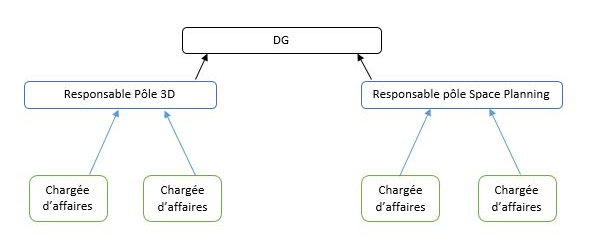
\includegraphics[scale=0.8]{organigramme.png}
\caption{Organigramme de l'entreprise}
\label{organigrammeImg}
\end{figure} 

\subsection{Domaine d'expertise}
Sp�cialis�e dans la d�finition, la conception et l'appropriation des espaces. UrbaProd est pr�sente tout  au long du cycle de vie du processus d'optimisation et de conception des lieux afin d'am�liorer la disposition  des collaborateurs :
\begin{itemize}
                                 \item En amont pour le recueil des besoins et le cadrage strat�gique.
                                 \item Puis pour la conception et la r�alisation des plans des espaces.
                                 \item Enfin pour la gestion et le pilotage de mobilit� et l'ing�nierie de transfert.
                               \end{itemize}
Les missions d' "UrbaProd" incluent :
\begin{itemize}
  \item Audit et programmation - Concept et charte d'am�nagement - Etudes et space planning.
  \item Prospective - Management de projet - Conduite du changement.
  \item Architecture d'int�rieur - Prescription mobilier - Conduite de travaux - OPC.
  \item Pilotage et gestion de la mobilit� - Ing�nierie de transfert.
  \item Solutions num�riques de gestion et visualisation des espaces.
\end{itemize}
UrbaProd travaille et accompagne les processus d'am�nagements des grands comptes en France et en Europe, � savoir : EDF, Thales, Cartier, Danone, INPI, l'Or�al, Technicolor, Hachette Livre dont nous retrouvons les logos dans la figure \ref{refenrenceImg} :

\begin{figure}[!ht]
\centering

\includegraphics[scale=0.8]{reference.png}
\caption{Organigramme de l'entreprise}
\label{refenrenceImg}
\end{figure}

\section{Solutions existantes}
Il existe plusieurs solutions de gestion de relation client sur le march�. En examinant ces applications, nous citons les plus importantes :
\subsection{Version �diteur}
\begin{itemize}

\item
CRM de Fitnet Manager : Fitnet Avant-vente est l'outil de gestion commerciale de Fitnet Manager. Les solutions CRM et ERP existent c�tes � c�tes. Activ�es ensemble, elles fonctionnent de mani�re enti�rement int�gr�e. Fitnet Manager couvre ainsi l'ensemble du cycle de vie de l'activit� : depuis la prospection jusqu'� la facturation et l'analyse dans les reporting \cite{Fitnet}.

  \item
  Everwin CXM : c'est une solution qui vise les cabinets d'architectures, elle couvre plusieurs fonctionnalit�s citant � titre d'exemple :
  \begin{itemize}
    \item
    Base de donn�es de la soci�t� et des contacts avec gestion automatis�e de la t�l�prospection.
    \item
    Gestion des actions commerciales et des campagnes marketing.
    \item
    Agenda partag� et planning g�n�ral des collaborateurs.
  \end{itemize}

\end{itemize}
Cette solution est fond�e sur une technologie Client/Serveur sous windows avec une base de donn�es SQL Server.
il est disponible en mode SaaS ou licence et peut �tre coupl� aux ERP ERPEverwin SX et Everwin GX \cite{Everwin} .   La figure \ref{everwinImg} illustre l'ensemble des fonctionnalit�s couvertes par Everwin CXM.

\begin{figure}[!ht]\centering
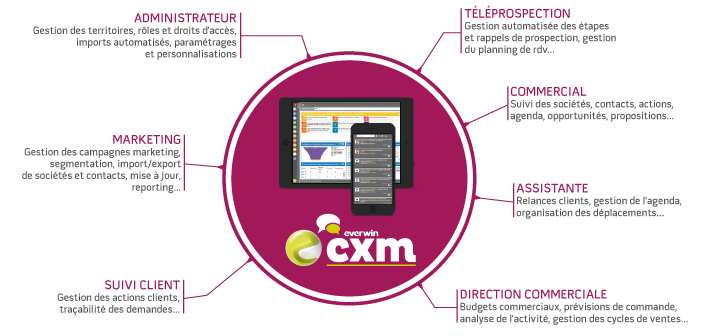
\includegraphics[scale=0.9]{everwinCXM.png}
\caption{Fonctionnalit�s offertes par Everwin CXM \cite{Everwin} }
\label{everwinImg}
\end{figure}

\subsection{Version libre}
\begin{itemize}
  \item Dolibar ERP/CRM : cette solution g�re les activit�s professionnelles ou associatives de point de vue contact, commandes, stock. Elle g�re aussi la gestion des projets et les avancements de leurs t�ches, et assure m�me la gestion de la ressource humaine.
	Dolibarr est disponible pour toute plate-forme puisqu'elle est d�velopp�e en PHP, MySQL ou encore PostgreSQL .
La figure \ref{dolibarr1Img} illustre l'architecture sur laquelle est bas�e la solution Dolibarr :

\begin{figure}[!ht]\centering
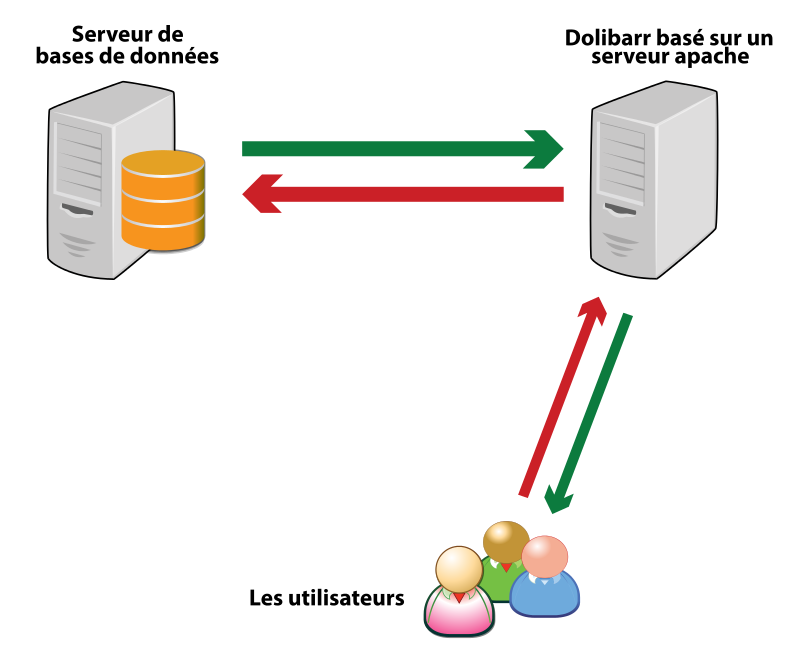
\includegraphics[scale=0.4]{Dolibarr1.png}
\caption{architecture Dolibarr \cite{Dolibarr} }
\label{dolibarr1Img}
\end{figure}

Pour les non connaisseurs dans le domaine du d�veloppement, il existe un auto-installateur qui se charge d'installer la solution avec tous ses pr�-requis (apache,mysql,php) \cite{Dolibarr}.
La figure \ref{dolibarr2Img} pr�sente l'�cran d'accueil de Dolibarr :

\begin{figure}[!ht]\centering
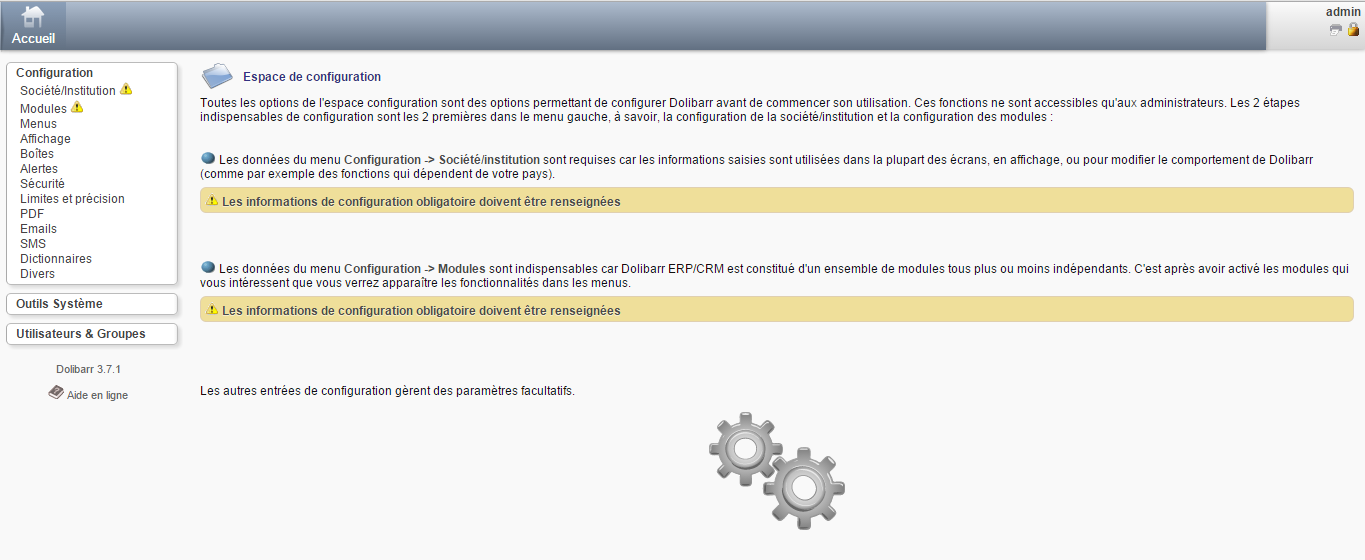
\includegraphics[scale=0.5]{accueil.png}
\caption{Ecran d'accueil de Dolibarr \cite{Dolibarr} }
\label{dolibarr2Img}
\end{figure}

\end{itemize}
\subsection{Etude comparative}
Le tableau \ref{compSolExt} pr�sente un comparatif entre les solutions existantes pr�sent�es pr�c�demment :

\begin{table}[!ht]\centering
  \centering
  \begin{tabular}{|c|c|c|c|c|c|}
    \hline
    % after \\: \hline or \cline{col1-col2} \cline{col3-col4} ...
    Solution & Payante &  Commentaire & Alertes & Mails & Accueil simple \\
    \hline
    Fitnet & oui  & non & oui & oui & non \\
    \hline
    Everwin CXM & oui  & non & oui & oui & non \\
    \hline
    Dolibarr & non  & non & oui & oui & non \\
    \hline
  \end{tabular}
  \caption{Comparatif entre les solutions existantes}\label{compSolExt}
\end{table}

Les applications �tudi�es, qu'elles soient en versions �diteurs ou m�me gratuites, et malgr� leurs adaptabilit�s et la diversit� de leurs fonctionnalit�s offertes, restes incapable de satisfaire les exigences de la soci�t�. En effet, elles n'int�grent pas un syst�me de commentaire et leur manipulation reste plut�t complexe compar�e � la solution � laquelle nous voulons aboutir.

\section{Objectif du projet}
Nous voulons offrir un meilleur service dans nos r�ponses aux collaborateurs � l'aide d'un v�ritable outil de gestion des demandes. Aujourd'hui nous visons de :
\begin{itemize}
  \item Faciliter la gestion des demandes.
  \item Rendre l'interaction entre les collaborateurs situ�s en Tunisie et en France plus fluide.
  \item Avoir un syst�me de notification dans l'application, par mail et par sms.
  \item Mesurer leur taux de satisfaction vis-�-vis des r�ponses aux demandes.
  \item Identifier le dysfonctionnement dans notre processus de travail.
  \item Avoir un suivi et une �valuation.
\end{itemize}

\section{Contexte m�thodologique du projet}
La grande �volution dans le domaine du d�veloppement est accompagn�e par une �volution des moyens assurant le bon fonctionnement de ce dernier. D'o� l'apparition des m�thodes agiles permettant d'organiser le cycle de d�veloppement des projets informatiques.

Les m�thodes agiles sont bas�es sur des principes communs d�finis dans l'Agile Manifesto qui est r�dig� par des experts dans ce domaine. Ils se reposent essentiellement sur une approche it�rative incr�mentale et adaptative �voluant en parall�le avec les besoins du client, afin de livrer un produit de qualit�.
Il existe plusieurs m�thodes agiles, � savoir, la m�thode  RUP \cite{RUP}, la m�thode XP \cite{XP}, la m�thode SCRUM \cite{SCRUM} et la m�thode RAD \cite{RAD}.

\subsection{Le choix de la M�thode Scrum}
Dans la majorit� des projets, il est difficile d'anticiper les attentes du client. Ceci nous oriente vers une approche it�rative permettant de s'adapter aux exigences du client au fur et � mesure de l'avancement du projet. Pour ce faire, nous choisi d'adopter la m�thode Scrum.
Aujourd'hui, Scrum est la m�thode agile la plus utilis�e. Elle permet de produire une solution de la plus haute qualit� dans des bref d�lais.
Cette m�thode est munie des atouts suivants :
\begin{itemize}
  \item Meilleur vue d'ensemble du projet : nous avons une vue globale sur l'avancement du projet par tous les membre des diff�rentes �quipes avec un traitement r�gulier des probl�mes rencontr�s durant chaque phase.
  \item Mise � jour des priorit�s : le client, qui n'est pas n�cessairement un informaticien, n'a pas toujours une vision compl�te sur le produit final. Pour cela, et gr�ce � la composition s�quentielle du contenu des sprints, il b�n�ficie d'une flexibilit� au niveau de la d�finition, de l'�volution des priorit�s et des s�quences d'activit�s.
  \item Qualit� du produit mise en avant : Cette m�thode se repose sur une �valuation r�guli�re du travail, ce qui permet un meilleur traitement des probl�mes (bug), une meilleure productivit� et un produit satisfaisant \cite{AvantageScrum}.
\end{itemize}

\subsection{Les r�les et les notions}
Les r�les dans Scrum :
\begin{itemize}
  \item Le product owner est le responsable du produit. Il est g�n�ralement le client et c'est lui qui exprime les diff�rentes sp�cifications fonctionnelles et leurs priorit�s.
  \item L'�quipe de d�veloppement est responsable de la r�alisation du livrable. Elle est constitu�e par l'entreprise et elle est auto-organis�.
  \item Le scrum master est le premier responsable sur le bon d�roulement des processus de la m�thode scrum.
\end{itemize}

Notion :
\begin{itemize}
  \item Sprint  : une it�ration de travail qui dure entre 15 et 30 jours.
  \item Le product backlog : repr�sente la liste des fonctionnalit�s r�dig�es par le product owner avec tous les correctifs et les am�liorations. Il est donc modifiable tout au long du projet. Le product backlog est pr�sent� sous forme d'items.
  \item Le sprint backlog : est l'ensemble des items planifi�s pour le sprint en cour \cite{SCRUM}.
\end{itemize}


\section*{Conclusion}
Dans ce chapitre, nous avons pr�sent� le cadre g�n�ral du travail, en commen�ant par la pr�sentation de l'entreprise Ellouze and Partners, passant par la probl�matique du projet, ainsi qu'une �tude des solutions existantes sur le march�. Et pour finir, nous avons pr�sent� la m�thode qui va guider notre travail tout au long du projet. Dans le chapitre suivant, nous introduisons les sp�cifications de notre projet.


%==============================================================================
\end{spacing}

\setcounter{chapter}{1}
\chapter{Capture,analyse et sp�cification des besoins}
\minitoc %insert la minitoc
\graphicspath{{Chapitre2/figures/}}

%\DoPToC

%==============================================================================
\pagestyle{fancy}
\fancyhf{}
\fancyhead[R]{\bfseries\rightmark}
\fancyfoot[R]{\thepage}
\renewcommand{\headrulewidth}{0.5pt}
\renewcommand{\footrulewidth}{0pt}
\renewcommand{\chaptermark}[1]{\markboth{\MakeUppercase{\chaptername~\thechapter. #1 }}{}}
\renewcommand{\sectionmark}[1]{\markright{\thechapter.\thesection~ #1}}

\begin{spacing}{1.5}
%==============================================================================
\section*{Introduction}

Ce chapitre repr�sente la case de d�part dans notre travail. En effet, nous analysons et sp�cifions les besoins du projet. Ensuite, nous identifions les diff�rents acteurs. Et enfin, nous mod�lisons le tout dans un diagramme de cas d'utilisation g�n�ral qui sera notre file conducteur durant la prochaine phase.

\section{�tude de l'existant}
	Pour soumettre une demande, nos collaborateurs chez G�nie des Lieux (GDL) � Paris ont quelques �tape � suivre :
\begin{itemize}
  \item T�l�chargement des fichiers.
Le t�l�chargement des fichiers Autocad avec extension DWG ou les fichiers 3DS sur lesquels nos collaborateurs � EllouzeAndPartners � Tunis vont travailler. Ce t�l�chargement s'effectue sur notre plate-forme priv�e qui nous g�n�re automatiquement un lien pour le t�l�chargement de ces fichiers ce qui nous m�ne � l'�tape suivante.
  \item Soumission du formulaire de demande.
Ensuite, les collaborateurs chez GDL remplissent un formulaire Excel pour d�tailler les missions � traiter dans cette demande. Les liens de t�l�chargement des fichiers t�l�charg�s sont soumis dans ce formulaire. Ce dernier est soumis via un mail.
  \item R�ponse des collaborateurs � tunis
L'�quipe d'EllouzeAndPartners r�pond � cette demande par un autre formulaire Excel pr�d�fini.
  \item Le suivi de la demande.
Ca se fait � travers l'Email, Skype ou par t�l�phone.
\end{itemize}

\section{Critique de l'existant }
\textcolor[rgb]{1.00,0.00,0.00}{\emph{Il faut Bien choisir les diagrammes ad�quats pour votre application. En g�n�ral, les
diagrammes obligatoires sont les diagrammes de cas d'utilisation, de classe et de
s�quence. Vous pouvez ajouter en plus le diagramme qui vous semble pertinent :
par exemple, pour une application sur plusieurs tiers, il est int�ressant de
montrer le diagramme de d�ploiement.}}




\section{Analyse des besoins}
Dans cette section, nous introduisons les diff�rents acteurs ainsi que les besoins fonctionnels et non fonctionnels.

\subsection{Les acteurs}
\begin{itemize}
  \item L'administrateur : c'est la personne charg�e d'affecter les diff�rents r�les et de g�rer les comptes.
  \item Collaborateur-FR : ils envoient les demandes depuis la France.
  \item Collaborateur-TN : ils assurent la r�ponse aux demandes.
\end{itemize}

\subsection{Les besoins fonctionnels}
\begin{itemize}
  \item La gestion des utilisateurs: l'administrateur doit disposer d'une interface permettant la gestion des utilisateurs, ainsi que la recherche et la gestion des r�les. En cas d'oubli, les utilisateurs peuvent changer leur mot de passe � travers leur adresse mail.
  \item La gestion des demandes: l'application doit permettre la cr�ation d'une demande, modifier ses donn�es, la gestion de ses diff�rentes phases ainsi que la recherche selon un ou plusieurs crit�res.
  \item La gestion des t�ches : l'application doit permettre la gestion compl�te des t�ches � faire dans chaque demande, i.e., la cr�ation, la modification et la suppression.
  \item La gestion des clients : l'application doit permettre l'ajout des clients,leur modification et leur suppression.
  \item La gestion des sites : l'application doit permettre l'ajout des sites relatifs � chaque client ainsi que leur modification et suppression.
  \item Extraction des donn�es : toutes listes d'utilisateurs, clients, sites, demandes, t�ches peuvent �tre extraite sous forme de fichier Excel, la demande est extraite sous la forme originale du formulaire utilis� auparavant par l'�quipe en France.
  \item L'envoie des notifications : l'application envoie automatiquement des notifications aux utilisateurs � chaque �v�nement important comme l'ajout ou la modification d'une demande ou l'ajout d'un nouveau commentaire.
\end{itemize}

\subsection{Les besoins non fonctionnels}
des notifications aux utilisateurs � chaque �v�nement important comme l'ajout ou la modification d'une demande ou l'ajout d'un nouveau commentaire.

\subsection{Planification du projet}
\subsubsection{Acteurs du projet}
Dans le tableau \ref{ActScrum} nous pr�sentons les diff�rents acteurs participants dans ce projet :
\begin{table}[!ht]
  \centering
  \begin{tabular}{|l|l|p{9cm}|}
    \hline
    % after \\: \hline or \cline{col1-col2} \cline{col3-col4} ...
    R�le & Acteur & Mission \\
    \hline
    �quipe & Anas BEN HAJ ALI & Conception,d�veloppement, tests unitaires, d�ploiement. \\
    \hline
    SCRUM master & Ons BEN CHEIKH & Assurer le bon d�roulement de la m�thode SCRUM. \\
    \hline
    Product owner & Aymen ELLOUZE & D�finir les fonctionnalit�s du produit et s'assurer de leur conformit�s. \\
    \hline
  \end{tabular}
  \caption{Les acteurs du SCRUM }\label{ActScrum}
\end{table}

\subsubsection{Backlog produit}
Il est �labor� par le product owner. Il comporte toutes les fonctionnalit�s du produit � d�velopper par l'�quipe de travail. Il est utilis� essentiellement pour planifier les releases. A la fin de chaque sprint, nous effectuons une mise � jour du backlog afin de prendre en compte les nouveaux besoins qui surviennent durant les sprints, et annuler les id�es non concluantes du d�part \cite{SCRUM}.
Dans le tableau \ref{backlogP}, nous pr�sentons le Backlog �tabli au d�but du projet.
\begin{table}[!ht]
  \centering
  \footnotesize
  \begin{tabular}{|p{4cm}|p{10cm}|c|}
    \hline
    % after \\: \hline or \cline{col1-col2} \cline{col3-col4} ...
    Nom & Description & Effort \\
    \hline
    Ajouter une mission & L'administrateur peut ajouter une mission. & 2 \\
    \hline
    Modifier une mission & L'administrateur peut modifier une mission. & 3 \\
    \hline
    Rechercher d'une mission & L'administrateur peut rechercher une mission par son titre. & 2 \\
    \hline
    Exporter les missions & L'administrateur peut exporter la liste des missions sous plusieurs formats. & 2 \\
    \hline
    Ajouter un client & Le collaborateur peut ajouter un client. & 2 \\
    \hline
    Modifier un client & Le collaborateur peut modifier un client. & 3 \\
    \hline
    Rechercher un client & L'administrateur peut rechercher un client. & 2 \\
    \hline
    Exporter les clients & L'administrateur peut exporter la liste des client sous plusieurs formats. & 2 \\
    \hline
    Affecter un site au client & Le collaborateur peut affecter un site au client. & 3 \\
    \hline
    Modifier un site & Le collaborateur peut modifier un site. & 3 \\
    \hline
    Rechercher un site & L'administrateur peut filtrer les sites. & 2 \\
    \hline
    Exporter les sites & L'administrateur peut exporter la liste des sites sous plusieurs formats. & 2 \\
    \hline
    Ajouter une cat�gorie & L'administrateur peut peut ajouter une cat�gorie de demande. & 2 \\
    \hline
    Modifier une cat�gorie & L'administrateur peut modifier une cat�gorie & 3 \\
    \hline
    Rechercher une cat�gorie & L'administrateur peut rechercher une cat�gorie. & 2 \\
    \hline
    Exporter les cat�gories & L'administrateur peut exporter la liste des cat�gories sous plusieurs formats. & 2 \\
    \hline
    Ajouter un utilisateur & L'administrateur peut ajouter un utilisateur. & 2 \\
    \hline
    Modifier un utilisateur & L'administrateur peut modifier un utilisateur. & 3 \\
    \hline
    D�sactiver un utilisateur & D�sactiver un utilisateur & 1 \\
    \hline
    Rechercher un utilisateur & L'administrateur peut filtrer les utilisateurs. & 2 \\
    \hline
    Exporter les utilisateurs & L'administrateur peut exporter la liste des utilisateurs sous plusieurs formats. & 3 \\
    \hline
    Initier une demande & Le collaborateur peut soumettre une demande. & 4 \\
\hline
    Modifier l'�tat d'une demande & Le collaborateur peut prendre en charge, livrer ou annuler une demande. & 2 \\
\hline
    Modifier une demande & Le collaborateur peut modifier une demande. & 3 \\
\hline
    Aimer une demande & Le collaborateur peut aimer une demande. & 4 \\
\hline
    ne pas aimer une demande & Le collaborateur peut ne pas aimer une demande. & 4 \\
\hline
    Commenter une demande & Le collaborateur peut commenter une demande. & 5 \\
\hline
    Rechercher une demande & L'administrateur peut filtrer les demandes selon plusieurs crit�res. & 2 \\
\hline
    Exporter la listes des  demandes en Excel. & Le collaborateur peut exporter la liste des demandes sous format Excel avec des informations restreintes. & 3 \\
\hline
    Exporter la listes des  demandes & L'administrateur peut exporter la liste des demandes sous diff�rents formats. & 2 \\
\hline
    Exporter une demande & Le collaborateur peut exporter la demande originale sous format Excel. & 3 \\
\hline
    Acc�der � un fil d'actualit�s & Le collaborateur peut acc�der � un fil d'actualit�s. & 5 \\
\hline
    �cran d'accueil & Le collaborateur peut acc�der � l'�cran d'accueil. & 4 \\
\hline
    Voir le feed-back graphique de l'avancement des demandes & Le collaborateur a un suivi graphique des demandes par mois. & 4 \\
\hline
    Envoyer une notification & Le syst�me doit notifier les utilisateurs � chaque nouvelle demande ou commentaire. & 5 \\
\hline
    Envoyer un mail de notification & Le syst�me doit �mettre un mail aux utilisateurs � chaque nouvelle demande. & 3 \\
\hline

  \end{tabular}
  \caption{Backlog du produit}\label{backlogP}
\end{table}

\subsubsection{Les sprints du projet}
Pour le bon d�roulement du projet, le travail sera d�coup� en sprint. Ces sprints sont �tabli � l'aide du backlog produit tout en respectant la priorit� des diff�rents modules.
Le tableau \ref{sprintP} pr�sente les sprints du projet :
\begin{table}[!ht]
  \centering
  \begin{tabular}{|c|l|c|}
    \hline
    % after \\: \hline or \cline{col1-col2} \cline{col3-col4} ...
    Sprint & description & dur�e \\
\hline
    sprint 0 & �tablissement du cahier de charge. & 3 semaines \\
\hline
    sprint 1 & Choix de la technologies et formation sur cette technologie. & 2 semaines \\
\hline
    sprint 2 & D�veloppement des modules gestion des missions et gestion des cat�gories. & 1 semaine \\
\hline
    sprint 3 & D�veloppement des modules gestion des clients et gestions des sites. & 1 semaine \\
\hline
    sprint 4 & D�veloppement du module gestion des utilisateurs. & 1 semaine \\
\hline
    sprint 5 & D�veloppement du module gestion des demandes. & 3 semaines \\
\hline
    sprint 6 & D�veloppement de ma partie exportation des demandes. & 1 semaine \\
\hline
    sprint 7 & D�veloppement de la gestion des commentaires et des "j'aimes". & 3 semaines \\
\hline
    sprint 8 & D�veloppement du module du notification. & 2 semaine \\
\hline
    sprint 9 & D�veloppement du fil d'actualit�. & 3 semaines \\
\hline
    sprint 10 & D�veloppement de l'�cran commun et du suivi graphique. & 1 semaine \\
\hline
    sprint 11 & Test et d�ploiement. & 1 semaine \\
    \hline
  \end{tabular}
  \caption{Les sprints du projet}\label{sprintP}
\end{table}

A la fin de chaque sprint, nous aurons un release qui sera examin� par le product owner afin de planifier les modifications et les �volutions � effectuer dans le sprint suivant.

\subsection{Sp�cification des besoins diagramme de cas d'utilisation global}
La figure \ref{useCaseGlobal} repr�sente le diagramme de cas d'utilisation global de l'application et les diff�rents acteurs qui interf�rent :

\begin{figure}[!ht]\centering
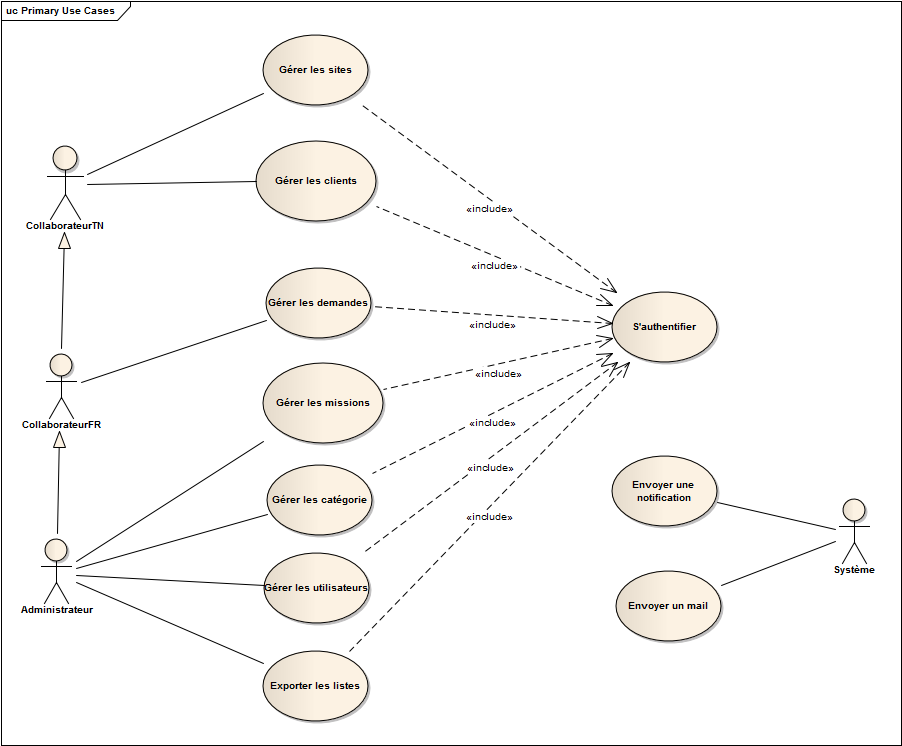
\includegraphics[scale=0.5]{PrimaryUseCases.png}
\caption{Diagramme de cas d'utilisation global}
\label{useCaseGlobal}
\end{figure}


\section*{Conclusion}
Dans ce chapitre, nous avons d�termin� les acteurs principaux dans notre projet ainsi que leur besoins. Ensuite, nous avons �tabli le Backlog produit sur lequel nous nous sommes appuy�s pour b�tir nos sprints.
Cette �tude sera notre base de travail dans le restant du chemain � savoir : la conception et la r�alisation de notre projet.
Dans le chapitre suivant nous allons exposer notre vue conceptuelle vis-�-vis du projet.





%==============================================================================
\end{spacing}


\setcounter{chapter}{2}
\chapter{Etude conceptuelle}
\minitoc %insert la minitoc
\graphicspath{{Chapitre3/figures/}}

%\DoPToC
%==============================================================================
\pagestyle{fancy}
\fancyhf{}
\fancyhead[R]{\bfseries\rightmark}
\fancyfoot[R]{\thepage}
\renewcommand{\headrulewidth}{0.5pt}
\renewcommand{\footrulewidth}{0pt}
\renewcommand{\chaptermark}[1]{\markboth{\MakeUppercase{\chaptername~\thechapter. #1 }}{}}
\renewcommand{\sectionmark}[1]{\markright{\thechapter.\thesection~ #1}}

\begin{spacing}{1.2}

%==============================================================================
\section*{Introduction}
phrase introductive

\section{Architecture physique}
Notre application est une application client/serveur qui dispose d'une architecture 3 tiers. C'est l'architecture la plus r�pandue dans les application web, dans laquelle la logique m�tier, l'acc�s et le stockage de donn�es et l'interface utilisateur sont maintenus chacune dans un module ind�pendant et pouvant �tre r�partis sur des plates-formes diff�rentes ou m�me regroup�s sur une seule machine. La figure \ref{archiTier} donne un aper�u sur cette architecture.

\begin{figure}[!ht]\centering
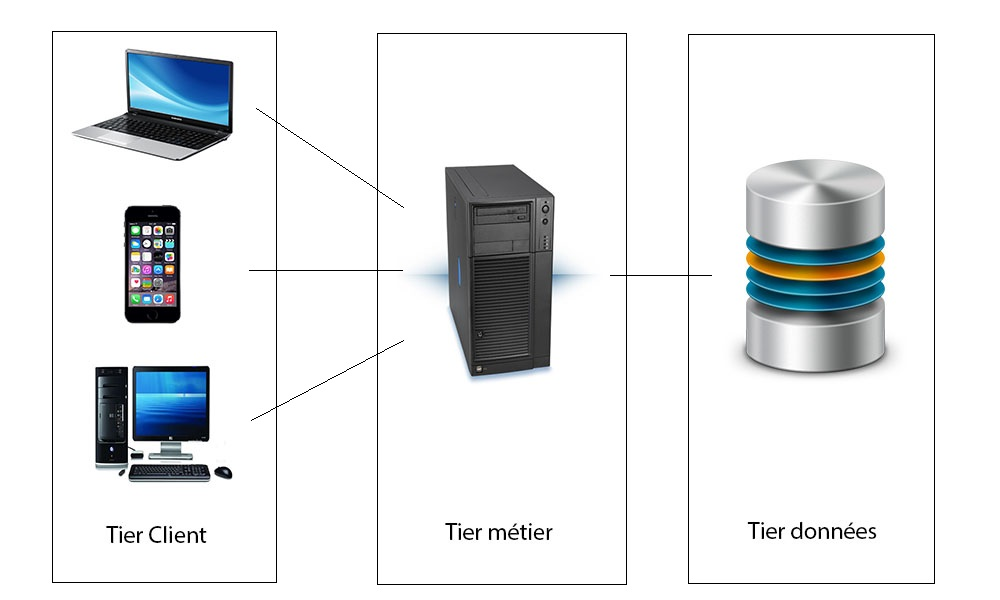
\includegraphics[scale=0.5]{archiTier.jpg}
\caption{Architecture physique}
\label{archiTier}
\end{figure}

\begin{itemize}
  \item Le client : ou la partie pr�sentation qui est dans notre cas le navigateur web (google Chrome, Mozilla Firefox etc).
  \item Le serveur d'application : ou la partie m�tier, elle est charg�e de faire des traitements sp�cifiques afin de r�pondre au requ�te HTTP du client venant de la couche pr�sentation.
  \item Le serveur de base de donn�es : dans notre cas c'est le syst�me de gestion de base de donn�es MySQL.
\end{itemize}





\section{Architecture logicielle}
Maintenant, nous pr�sentons l'architecture applicative de notre application, sa structure en couche et leur description, � savoir, la couche pr�sentation, la couche service et la couche acc�s � la base de donn�es. Nous mod�lisons par la figure \ref{archiAppl} ces couches ainsi que les diff�rents invocations entre eux.

\begin{figure}[!ht]\centering
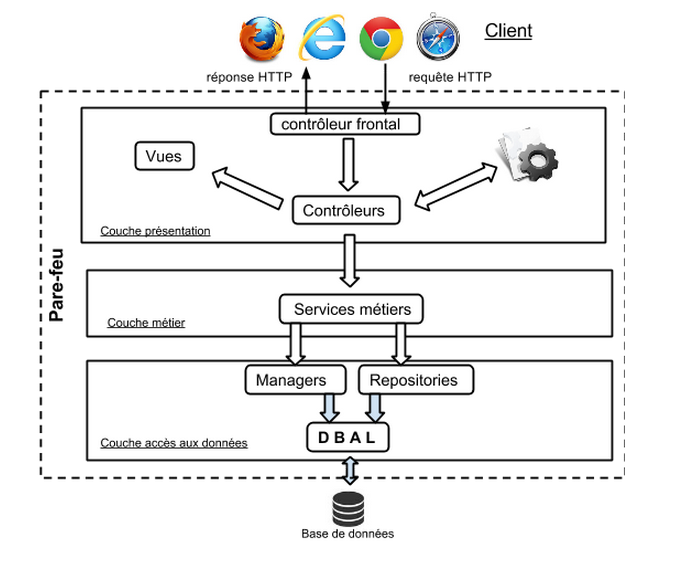
\includegraphics[scale=1]{archiApplicative.png}
\caption{Architecture applicative de la solution}
\label{archiAppl}
\end{figure}

\begin{itemize}
  \item La couche pr�sentation : elle repr�sente le contact de l'utilisateur avec l'application, elle lui permet le pilotage et la configuration de l'application. Elle invoque le service m�tier ad�quat � la requ�te du client et lui retourne le r�sultat. Cette couche est compos�e de :
      \begin{itemize}
        \item Contr�leur frontal : il repr�sente le point d'entr�e de notre application.
        \item Contr�leurs : ils d�cident selon la requ�te du client et les configuration du syst�me, quel service sera invoqu� et quelle vue sera rendu, autrement dit, ils orchestrent les diff�rents �l�ments.
        \item Vues : le r�sultat de la requ�te de l'utilisateur est r�cup�r� et traduit en HTML et Javascript puis renvoy� au client sous forme de vue selon la charte graphique utilis�e dans l'application.
      \end{itemize}
  \item La couche m�tier : c'est l'�l�ment qui englobe la logique m�tier et ses traitements sp�cifiques. Elle est invoqu�e via les contr�leurs pour traiter les requ�tes client.
  \item La couche acc�s au base de donn�es : cette couche assure la communication avec la source de donn�es afin d'assurer la s�paration entre la logique m�tier et la logique acc�s au donn�es.
	  Elle est compos�e de :
        \begin{itemize}
          \item Managers : Ils assurent la persistance des donn�es dans la base de donn�es.
          \item Repositories : Ils assurent l'extraction des donn�es de la base de donn�es.
          \item Database Abstract Layer DBAL : Elle offre un acc�s facile et rapide � la base de donn�es [W5]. Elle procure plusieurs service  : l'insertion, la mise � jour, la suppresion et la lecture des donn�es.
Elle est caract�ris�e par un Object Relation Mapping (ORM) qui traduit  les tables de la base en objets facilement manipulable.
        \end{itemize}
\end{itemize}
Dans les paragraphes pr�c�dents, nous avons pr�sent� les mod�les architecturals de notre application ce qui nous m�nera � la partie conception dans la quelle nous allons d�tailler nos diagrammes de cas d'utilisation, pr�senter les diagrammes de classes ainsi que quelques exemple des cas d'activit� les plus importants.



\section{Raffinement des diagrammes des cas d'utilisations}
Dans cette partie, nous d�cortiquons les cas d'utilisation vus dans le chapitre pr�c�dent d'une fa�on plus d�taill�e afin de clarifier le fonctionnement de notre syst�me.
\subsection{module gestion de demande}
Ce module regroupe toutes les rubriques de gestion d'une demande.
La cr�ation des demandes est conduite par les collaborateurs en France. Les collaborateurs � Tunis auront une visibilit� sur les d�tails du travail � faire ainsi que sur les interactions qu'ils peuvent effectuer avec la demande. La figure \ref{useCaseGestionDemande} montre le diagramme de cas d'utilisation de gestion d'une demande.

\begin{figure}[!ht]\centering
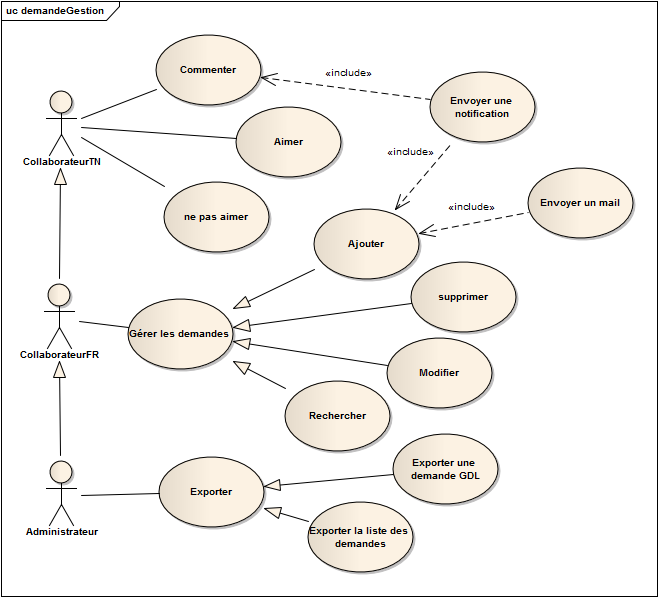
\includegraphics[scale=0.5]{demandeGestionFinal.png}
\caption{Diagramme de cas d'utilisation Gestion d'une demande}
\label{useCaseGestionDemande}
\end{figure}
\begin{itemize}
  \item Description du cas d'utilisation : ajout d'une demande \\
  Le tableau 3. d�crit le cas d'utilisation "ajout d'une demande".

\begin{table}[!ht]
	\centering
	\begin{tabular}{|l|p{11cm}|}	
			\hline
			Titre 		&	Ajouter une nouvelle demande.	\\
\hline			
Acteur		&   Collaborateur FR.   \\
\hline		
	R�sum�		&	Le collaborateur peut ajouter une nouvelle demande en sp�cifiant les diff�rentes informations relatives � son ex�cution, e.g. date limite, client, format du rendu. \\
\hline
			Pr� condition		&	Le collaborateur doit �tre authentifi�. \\
\hline		
	Sc�nario principal	 	& \begin{enumerate}
                            \item Le collaborateur se rend dans la page d'accueil ou sur la page de la  liste des demandes.
                            \item Le collaborateur affiche le pop-up du formulaire de la demande.
                            \item Le collaborateur saisie les informations n�cessaires et appuie sur cr�er.
                            \item Le collaborateur joint les fichiers sur lesquels les collaborateur � Tunis vont travailler.
                            \item Le syst�me enregistre la demande.
                            \item Le syst�me �met une notification � tous les utilisateurs pour les informer de la nouvelle demande.
                            \item Le syst�me envoie un mail � tout les utilisateurs pour les informer de la nouvelle demande.
                            \item Le syst�me affiche un message de confirmation et le redirige vers la page d'accueil ou sur la page de la liste des demandes.
                            \end{enumerate}
  \\
\hline		
	Sc�nario d'exception		&	Erreur dans les informations saisies :
                                            \begin{itemize}
                                              \item Le syst�me affiche les messages d'erreur devant les champs concern�s.
                                              \item Nous reprenons depuis l'�tape 3.
                                            \end{itemize}

  \\
			\hline
	\end{tabular}
	\label{ajoutDemande}
	\caption{Ajout d'une demande}
\end{table}


\item Description du cas d'utilisation : commenter une demande\\
Le cas d'utilisation "ajout d'un nouveau commentaire" est d�crit dans le tableau \ref{ajtCommTab}.

\begin{table}[!ht]
  \centering
  \begin{tabular}{|l|p{10cm}|}
    \hline
    % after \\: \hline or \cline{col1-col2} \cline{col3-col4} ...
    Titre & Commenter une demande. \\
    \hline
    Acteur  & Collaborateur TN. \\
    \hline
    R�sum� & Afin d'intervenir dans le cycle de vie d'une demande ou de poser son point de vue, un collaborateur peut ajouter un commentaire tout en joignant des images. \\
    \hline
    Pr� condition & Le collaborateur doit �tre authentifi�. \\
    \hline
    Sc�nario principal & \begin{enumerate}
                           \item Le collaborateur se rend dans la file d'actualit� ou dans la vue d'une demande.
                           \item Le collaborateur saisie son commentaire.
                           \item Le collaborateur joint les images.
                           \item Le syst�me enregistre le commentaire.
                           \item Le syst�me affiche le nouveau commentaire.
                           \item Le syst�me place le collaborateur dans l'espace de commentaire afin qu'il puisse ajouter un autre.
                         \end{enumerate}
     \\
    \hline
    Sc�nario d'exception & Erreur dans le type des fichiers joint :
                                \begin{itemize}
                                  \item le syst�me affiche l'impossibilit� de charger ce type de fichier ( fichier.php ) .
                                  \item on se rend depuis l'�tape 4.
                                \end{itemize}
                                 \\
    \hline
  \end{tabular}
  \caption{Ajouter un nouveau commentaire}\label{ajtCommTab}
\end{table}

\end{itemize}

\subsection{module gestion des utilisateurs}
Ce sont les diff�rentes fonctionnalit�s offertes afin de g�rer les collaborateurs au sein de l'application.
Le figure \ref{useCaseUser} illustre le diagramme de cas d'utilisation de gestion des utilisateurs.

\begin{figure}[!ht]\centering
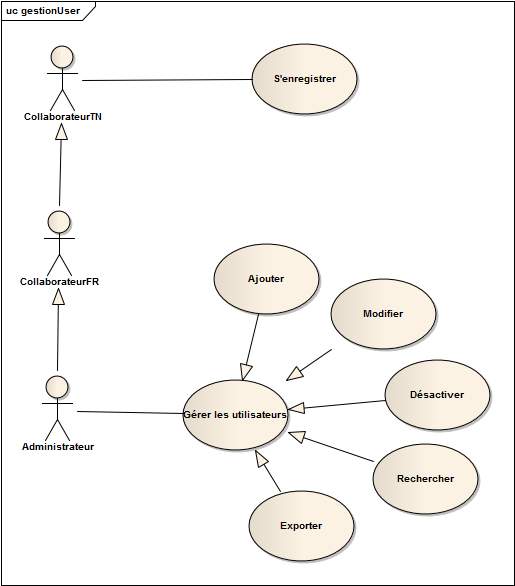
\includegraphics[scale=0.5]{utilisateurGestionFinal.png}
\caption{Diagramme de cas d'utilisation gestion utilisateurs}
\label{useCaseUser}
\end{figure}

\begin{itemize}
  \item Description du cas d'utilisation : ajout d'un utilisateur \\
  Ce cas est d�crit par le tableau \ref{addUserTab}.

\begin{table}[!ht]
  \centering
  \begin{tabular}{|l|p{10cm}|}
    \hline
    % after \\: \hline or \cline{col1-col2} \cline{col3-col4} ...
    Titre & Ajout d'un utilisateur. \\
    \hline
    Acteur & Administrateur , Collaborateur. \\
    \hline
    R�sum� & Ce cas permet � l'administrateur de bien organiser les utilisateurs de l'application en leur affectant les diff�rents r�les. En fait, chaque r�le permet � son utilisateur des acc�s sp�cifiques et limit�s. \\
    \hline
    Pr� condition & Un administrateur est authentifi�. \\
    \hline
    Sc�nario principal & \begin{enumerate}
                           \item L'administrateur envoie la vue d'enregistrement � un collaborateur.
                           \item Le collaborateur saisi ses informations.
                           \item Le syst�me enregistre ces informations.
                           \item Le syst�me met � jour la liste des collaborateurs.
                           \item L'administrateur affecte les r�les de ce collaborateur et l'active pour qu'il puisse acc�der � l'application.
                         \end{enumerate}
     \\
    \hline
    Sc�nario d'exception & L'utilisateur essaie de s'inscrire avec une adresse mail existante :
                        \begin{itemize}
                          \item Le syst�me affiche l'erreur pr�s du champs concern�.
                          \item Le processus reprend depuis l'�tape 2.
                        \end{itemize}
                         \\
    \hline
  \end{tabular}
  \caption{Ajout d'un utilisateur}\label{addUserTab}
\end{table}

\end{itemize}

\subsection{Module gestion des param�tres de la demandes.}
Cette partie regroupe les diff�rentes fonctionnalit�s qui servent � param�trer les demandes. Vue que les missions effectu�es dans l'entreprise sont connues d'avance, c'est le directeur de l'entreprise qui est charg� de les pr�d�finir. Les clients et leurs sites sont d�finis au pr�alable comme ils peuvent �tre d�finis lors de la soumission d'une nouvelle demande.
La figure \ref{useCaseParametre} montre ces diff�rents cas d'activit�s.

\begin{figure}[!ht]\centering
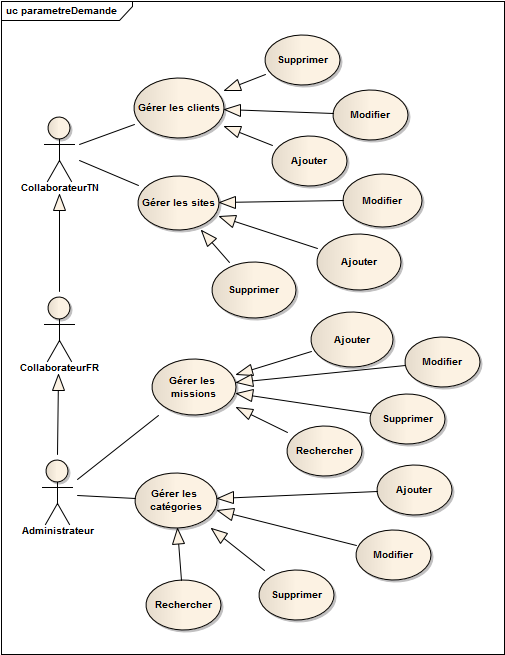
\includegraphics[scale=1]{GestionParametreFinal.png}
\caption{Diagramme d'utilisation du param�trage d'une demande}
\label{useCaseParametre}
\end{figure}

\begin{itemize}
  \item Description du cas d'utilisation : ajout d'un nouveau site \\
  Ce cas d'utilisation est d�crit par le tableau \ref{AjoutSitTab}.

\begin{table}[!ht]
  \centering
  \begin{tabular}{|p{4cm}|p{9cm}|}
    \hline
    % after \\: \hline or \cline{col1-col2} \cline{col3-col4} ...
    Titre & Ajout d'un nouveau site. \\
    \hline
    Acteur & Collaborateur. \\
    \hline
    Description & La plupart des clients sont de grande entreprise donc ils poss�dent plusieurs sites et � chaque fois nous travaillons sur l'un d'eux. C'est la raison pour laquelle l'affectation du client seulement n'est pas suffisante. Nous devons donc, dans chaque demande, pr�ciser le site sur lequel nous travaillons. \\
    \hline
    Pr� condition & Le collaborateur doit �tre authentifi�. \\
    \hline
    Sc�nario principal & \begin{enumerate}
                           \item Le collaborateur se rend sur la page des sites.
                           \item Le collaborateur affiche le pop-up de l'ajout d'un site.
                           \item Le collaborateur indique le client.
                           \item Le collaborateur saisi les informations du site.
                           \item Le syst�me enregistre le nouveau site.
                         \end{enumerate}
     \\
    \hline
    Sc�nario alternatif & \begin{enumerate}
                            \item Le collaborateur saisi les informations d'une nouvelle demande.
                            \item Le collaborateur ne trouve pas le site voulu.
                            \item Nous reprenons d�s l'�tape 2 du sc�nario principal.
                          \end{enumerate}
     \\
    \hline
    Sc�nario d'exception & Le collaborateur ne trouve pas de client disponible :
    \begin{itemize}
      \item Le syst�me affiche l'erreur indiquant l'absence des client.
      \item Le collaborateur doit ajouter un nouveau client.
      \item Le sc�nario reprend depuis l'�tape 1.
    \end{itemize}
     \\
    \hline
  \end{tabular}
  \caption{Ajout d'un nouveau site}\label{AjoutSitTab}
\end{table}
\end{itemize}

\subsection{Module exportation des donn�es}
Ce module permet en fait plusieurs types d'exportation.
Tout d'abord, il permet l'extraction de la demande sous sa forme originale adapt�e avant le d�veloppement de notre application (comme indiqu� dans l'annexe 1).
Pour le suivi du travail ou un contr�le quotidien, nous pouvons exporter les donn�es dans des fichiers Excel.
Vue la nature des autres activit�s de l'entreprise, nous aurons besoins aussi d'autre types de flux d'information i.e. JSON et XML.
La figure \ref{useCaseExporter} met en �vidence ces cas d'utilisation.

\begin{figure}[!ht]\centering
\includegraphics[scale=0.6]{ExportDonn�esFinal1.png}
\caption{Diagramme de cas d'utilisation exportation des donn�es}
\label{useCaseExporter}
\end{figure}

\begin{itemize}
  \item Description du cas d'utilisation : exporter la liste des demandes.\\
  Le tableau \ref{expListTab} d�crit ce cas d'utilisation .

\begin{table}[!ht]
  \centering
  \begin{tabular}{|l|p{11cm}|}
    \hline
    % after \\: \hline or \cline{col1-col2} \cline{col3-col4} ...
    Titre & Exporter la liste des demandes. \\
    \hline
    Acteur & Administrateur. \\
    \hline
    Description & Afin de faire le suivi du travail dans l'entreprise, ou de facturer le travail effectu� par l'�quipe, le directeur a besoin d'une vue globale sur les demandes. \\
    \hline
    Pr� condition & Un administrateur est authentifi�. \\
    \hline
    Sc�nario principal & \begin{enumerate}
                           \item L'administrateur se rend sur la page d'administration.
                           \item L'administrateur affiche les demandes.
                           \item L'administration choisit le type de flux de sortie.
                           \item L'administrateur exporte les donn�es.
                         \end{enumerate}
     \\
    \hline
  \end{tabular}
  \caption{Exporter la liste des demandes}\label{expListTab}
\end{table}
Apr�s la pr�sentation des diff�rents diagrammes de cas d'utilisation, nous d�taillons dans la section suivante, la conception de notre application � travers les diagrammes structurels et comportementaux.
\end{itemize}

\section{Diagrammes structurels}
\subsection{Diagramme de paquetages}
Pour une application maintenable, nous avons opt� pour la division en packages. Le package est un regroupement de classe ou d'�l�ments de mod�lisation de pr�f�rence de m�me type. Donc ce diagramme met en �vidence l'organisation de notre travail \cite{Package}.
La figure \ref{paquetageDiagram} pr�sente le diagramme de packetages.

\begin{figure}[!ht]\centering
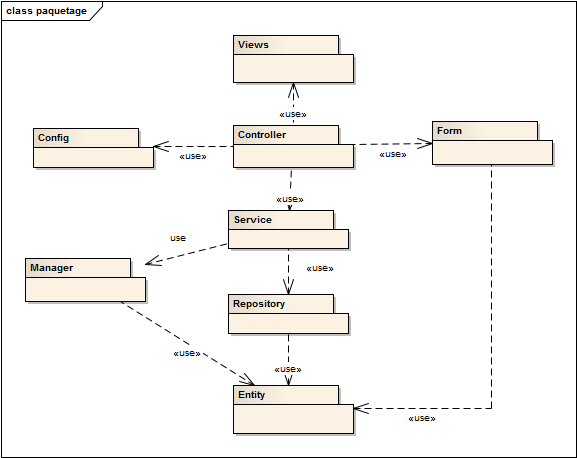
\includegraphics[scale=0.7]{paquetageFinal.png}
\caption{Diagramme de paquetage}
\label{paquetageDiagram}
\end{figure}

En fait, ce diagramme met en �vidence le mod�le Model View Controller (MVC) \cite{MVC}, � travers les packages Views, Controller, Repository, Manager et Entity.
Entity : il regroupe les entit�s de notre application.
Manager : il regroupe les �l�ments g�rant la persistance dans la base de donn�es.
Repository : il regroupe les �l�ments responsable de l'extraction des donn�es de la base de donn�es.
Views : il regroupe les vues de notre application. Il repr�sente le contacte directe avec l'utilisateur.
Controller : il regroupe les contr�leurs de l'application. Ils jouent le r�le de chef d'orchestre en appellant le mod�le et en le redirigent vers la vue convenue.
Il existe aussi d'autre packages :
Service : il regroupe les services li�s � notre application.
Form : il regroupe les formulaires de l'application mod�lis�s par des classes.
Config : il contient le routage de l'application et les services.

\subsection{Diagramme de classes}
\begin{itemize}
  \item Le mod�le du domaine.\\
  La figure \ref{ModlDmnClass} illustre le mod�le du domaine de l'application web avec les diff�rentes d�pendances.

\begin{figure}[!ht]
\centering
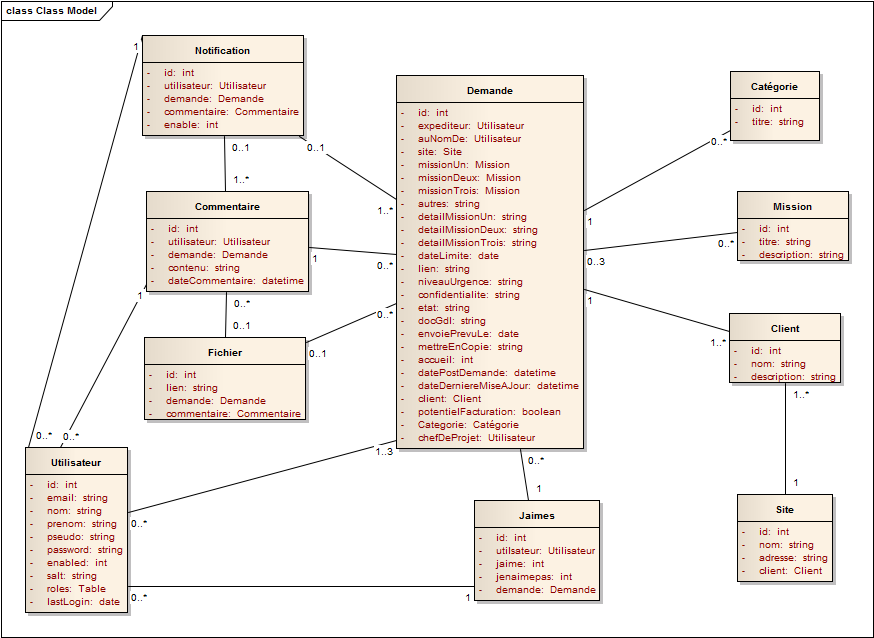
\includegraphics[scale=0.6]{diagrammeClasses.png}
\caption{Le mod�le du domaine}
\label{ModlDmnClass}
\end{figure}

Ce sont les diff�rentes entit�s qui constituent le mod�le du domaines.
Elles repr�sentent la fa�on avec laquelle les donn�es sont stock�s dans la base.	
Dans le tableau 3.6, nous repr�sentons le r�le de chacune de ces entit�s.
 
\begin{table}[!ht]
  \centering
  \begin{tabular}{|l|p{11cm}|}
    \hline
    % after \\: \hline or \cline{col1-col2} \cline{col3-col4} ...
    Entit� & Description \\
    \hline
    Utilisateur & Elle repr�sente un collaborateur chez l'entreprise, elle contient les informations de chacun d'eux et pr�cise leur r�le dans l'entreprise. \\
    \hline
    Demande & Cette entit� repr�sente les exigences du client transmises par nos collaborateurs en France. Les exigences sont pr�d�finies et repr�sent�es par les missions.  \\
    \hline
    Commentaire & Ce sont les diff�rents impressions, interrogations, ou d�clarations que laissent les utilisateurs � propos d'une demande. Ils peuvent �tre accompagn�s par des photos. \\
    \hline
    Fichier & Il peut �tre un fichier attach� � une demande, une image dans commentaire ou l'image d'un utilisateur. \\
    \hline
    Notification & C'est un signal envoy� au utilisateur pour leur notifier d'un nouvel �v�nement. \\
    \hline
    Jaime & Ceux sont les impressions des collaborateurs � propos d'une demande. Soit ils l'aiment soit ils ne l'aiment pas. \\
    \hline
    Cat�gorie & La cat�gorie d'une demande sert dans la facturation. \\
    \hline
    Mission & C'est une t�che que nous pouvons effectuer dans notre entreprise. \\
    \hline
    Client & Elle repr�sente nos clients. \\
    \hline
    Site & Elle repr�sente o� se situe le locale de l'entreprise avec laquelle nous traitons.  \\
    \hline
  \end{tabular}
  \caption{Descriptif des entit�s de l'application}\label{entityTab}
\end{table}

 \item Diagramme de classe des contr�leurs.\\
 La figure \ref{ctrlClass} montre le diagramme de classe des contr�leurs.
 
\begin{figure}[!ht]
\centering
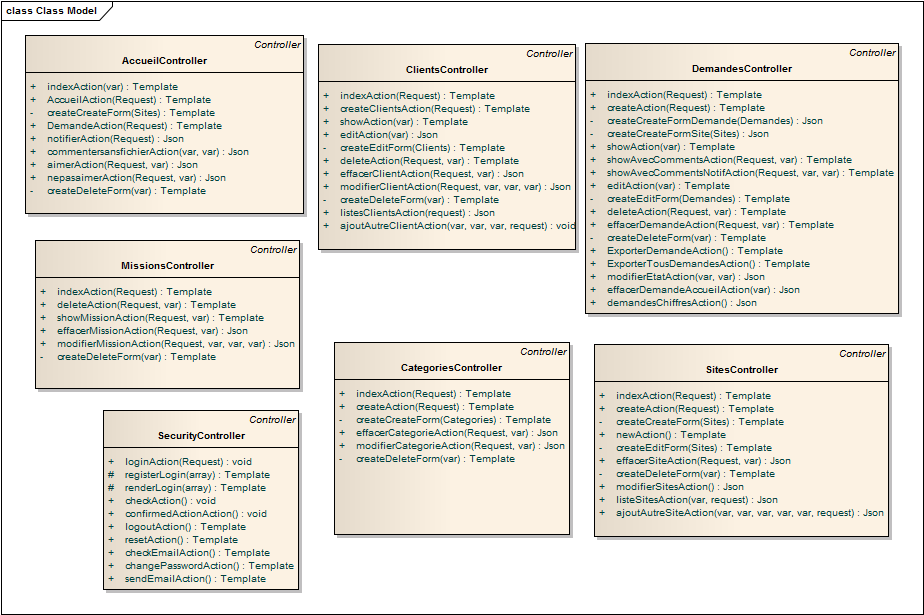
\includegraphics[scale=0.5]{controlerClass.png}
\caption{Le mod�le du domaine}
\label{ctrlClass}
\end{figure} 

 Les contr�leurs sont invoqu�s selon les routes, chaque route pointe vers une seule m�thode d�un contr�leur bien sp�cifique. Donc une seule route ne peut pas invoquer plusieurs actions simultan�ment.
\end{itemize}

\section{Diagramme comportementaux}
\subsection{Diagrammes de s�quences}
\begin{itemize}
  \item Diagramme de s�quence du cas : ajouter une demande. \\
  Dans la figure 4.10, nous pr�sentons la cr�ation d�une demande � travers les principales interactions entre les diff�rents �l�ments de l�application.
L�exemple trait� est le cas d�un collaborateur qui cr�e une demande avec des donn�es correctes.

\begin{figure}[!ht]
\centering
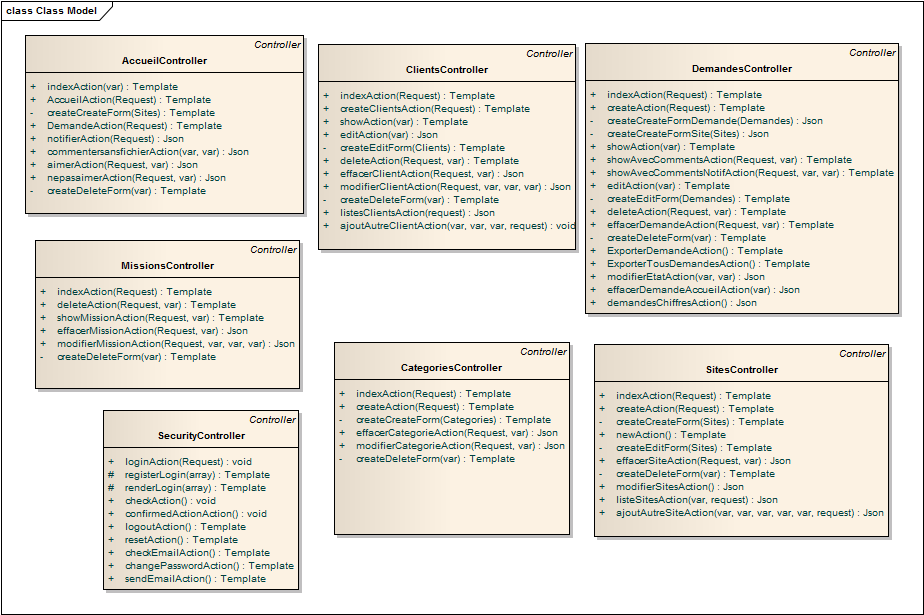
\includegraphics[scale=0.5]{controlerClass.png}
\caption{Le mod�le du domaine}
\label{ctrlClass}
\end{figure} 
  
  
  \item 
\end{itemize}


\section*{Conclusion}
Voil�.

%==============================================================================
\end{spacing}


\setcounter{chapter}{3}
\chapter{R�alisation}
\minitoc %insert la minitoc
\graphicspath{{Chapitre4/figures/}}

%\DoPToC
%==============================================================================
\pagestyle{fancy}
\fancyhf{}
\fancyhead[R]{\bfseries\rightmark}
\fancyfoot[R]{\thepage}
\renewcommand{\headrulewidth}{0.5pt}
\renewcommand{\footrulewidth}{0pt}
\renewcommand{\chaptermark}[1]{\markboth{\MakeUppercase{\chaptername~\thechapter. #1 }}{}}
\renewcommand{\sectionmark}[1]{\markright{\thechapter.\thesection~ #1}}

\begin{spacing}{1.5}

%==============================================================================
\section*{Introduction}

Dans les chapitres pr�c�dents, nous avons d�taill� la m�thodologie suivie durant notre travail ainsi que la conception de notre application. Dans l'�tape suivante, nous proc�dons � la pr�sentation de notre environnement de travail et les diff�rentes technologies utilis�es pour enfin terminer avec les principales fonctionnalit�s r�alis�es et leurs interfaces.

\section{Environnements de travail et choix techniques}
Cette section met l'accent sur les logiciels utilis�s durant ce travail. Puis nous abordons	les choix des diff�rentes technologies mises en place.

\subsection{Environnements de travail}
Les principaux logiciels utilis�s sont :
\begin{itemize}
  \item Netbeans 8.0.2 : c'est un environnement de d�veloppement int�gr� (IDE)  qui supporte plusieurs langage e.g., php, java, c.
C'est un produit oracle qui est maintenu � jour pour supporter les
derniers technologies et framework les plus utilis�s \cite{Netbeans}.
  \item Microsoft Office : World 2013 pour la r�daction du cahier de charge et Excel 2013 pour l'exportation des diff�rents informations dans notre application.
  \item Adobe Photoshop CS6 : utilis� pour le traitement des images utilis�es tout le long du stage que ce soit dans le rapport, �laboration du cahier de charge ou le d�veloppement de l'application.
  \item WampServer 2.5 : pour la simulation locale du serveur web, nous avons choisi ce serveur pour la facilit� du partage des donn�es dans un serveur local ou � distance c'est � dire pour des utilisateurs de l'ext�rieur de notre r�seau.
  \item Mozilla Firefox, Google Chrome : nous avons effectu� le test des vues dans ces navigateurs sur un �cran pc 23 pouces et sur une tablette Galaxy Tab 4 de Samsung pour une qualit� optimale.
  \item Git et Github : afin de garder un trace de notre travail, d'avoir la possibilit� d'un retour en arri�re en cas de probl�me, nous avons utilis� l'outil de versionning Git qui offre la possibilit� de sauvegarder notre travail avec un simple "commit" et permet m�me d'effectuer des sauvegardes en ligne avec le "push".
La figure \ref{commitImg} et \ref{contributionImg} pr�sentent l'interface du Github avec quelques "commit" et toutes les contributions effectu�es pendant notre travail.

\begin{figure}[!ht]
\centering
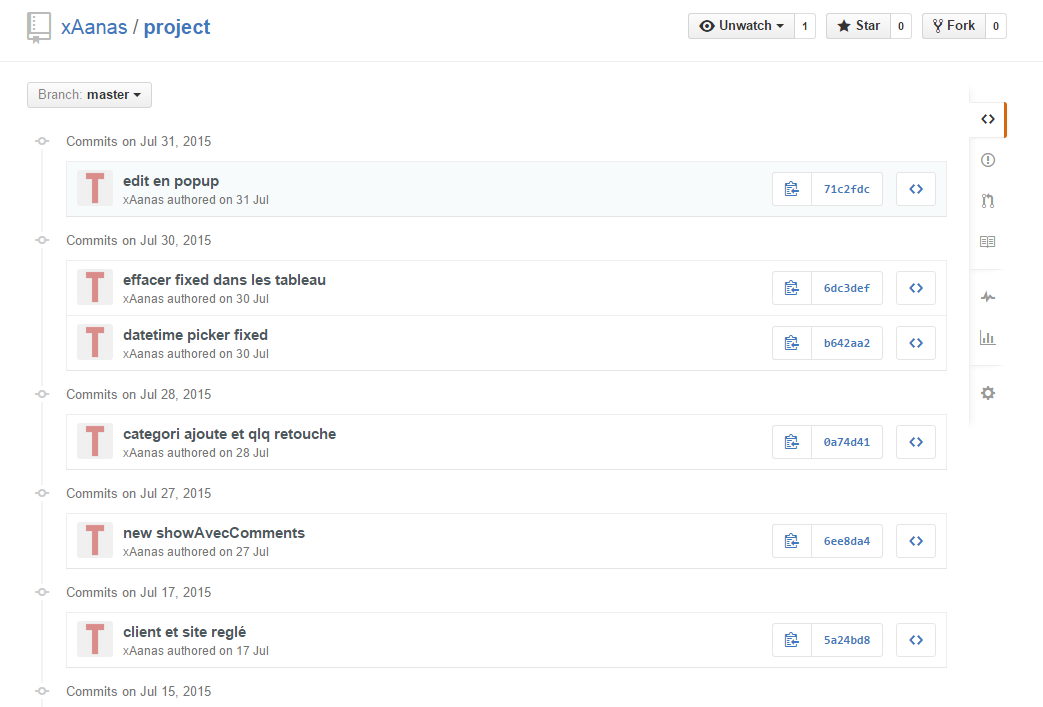
\includegraphics[scale=0.6]{commit.png}
\caption{Commits pendant le mois de Juillet}
\label{commitImg}
\end{figure}

\begin{figure}[!ht]
\centering
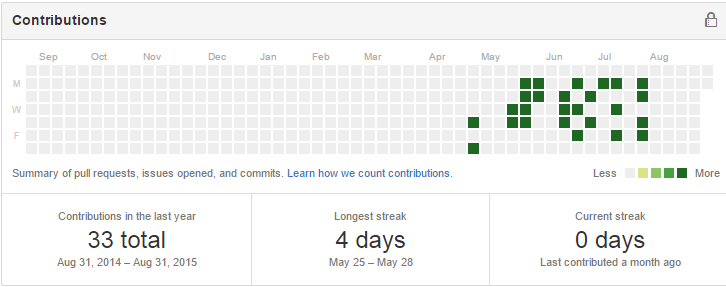
\includegraphics[scale=0.7]{contributions.png}
\caption{Toutes les contributions}
\label{contributionImg}
\end{figure}
  \item Sublime Text 2 : pour le d�veloppement ou la modification de quelques scripts.
  \item Miktex : pour la g�n�ration du rapport.
\end{itemize}

\subsection{Technologies}
Durant notre travail, plusieurs choix technique ont �t� faits. Dans ce qui suit, nous illustrons les plus importants :\\
\begin{itemize}
  \item Le Framework Symfony2.\\
	Une exigence du client d�s le d�but du projet, �tait de travailler avec le langage PHP sur une base de donn�es MySQL.
L'id�e du client �tait de travailler avec du PHP natif �tant donn�e qu'un Framework n'est pas indispensable pour le d�veloppement d'une application Web mais apr�s l'�laboration du cahier de charge et vue le volume du travail demand� et la nature des fonctionnalit�s, il serait impossible de terminer le projet dans les d�lais. Le recourt � un Framework PHP devient indispensable. Ses b�n�fices ne se limitent pas au gain �norme du temps que nous aurions mais aussi de la structuration du projet. Nous aurons un cadre de travail conforme au r�gles du m�tier qui nous fournira un code maintenable, �volutif et des librairies r�utilisables facilitant plusieurs t�ches.
Il nous permet donc d'�viter les anti-pattern comme don't repeat yourself (DIE), qui consiste � ne pas r�inventer la roue et mettre en oeuvre des composants existants.
Parmi les Framework gratuits sur le march� nous avons identifi� les trois les plus utilis�es et qui sont Laravel, Zend2 (ZF2) et Symfony2 (SF2).
Vue que Laravel est encore nouveau et immature, le choix s'est limit� entre ZF2 et SF2.
Ces deux Framework sont matures et stables. Ils adaptent une architecture similaire, la seule diff�rence frappante entre ses deux leaders est la richesse de la documentation qui a jou� en faveur du SF2 et surtout sa communaut� tr�s active \cite{Sf2vsZf2}.
En effet, avec le Cookbook symfony2 \cite{cookBook} et la grande vari�t� des tutoriels �a devient facile de g�rer ses erreurs et r�pondre � nos besoins.
D'autre part, SF2 est dot� de plusieurs outils tels que Doctrine2 qui est l'ORM de SF2, il offre plusieurs fonctionnalit�s facilitant la manipulation de la base de donn�es et communique directement avec la DBAL \cite{Dbal}. Le moteur de template TWIG qui nous garantit un code net et propre s�parant le code php du code html et Javascript.
  \item Composer.\\
	C'est le gestionnaire de d�pendance d�di� au PHP. Il facilite l'import des bundles afin de les r�utiliser et permet �galement de maintenir notre application � jour � travers un simple update (semblable au MAVEN pour le langage Java).
  \item Bundles.\\
	Ce sont des modules d�velopp�s par la communaut� Symfony pour �viter de r�inventer la roue. En effet, leur int�gration est facile gr�ce au Composer qu'on vient de d�finir dans le paragraphe pr�c�dant et permettent de gagner �norm�ment de temps \cite{Bundles}.
  \item Highcharts.\\
 	Pour un rendu simple et clair des donn�es nous avons eu recours � Highcharts qui est une biblioth�que Javascript sp�cialis�e dans la repr�sentation graphique. Ayant la possibilit� de consommer du JSON et d'exporter des sch�mas sous format PDF ou m�me en image, cette biblioth�que a pris le dessus sur tous ses concurrents, e.g. Charts js ou encore D3js qui n'assurent pas l'exportation des donn�es \cite{Highcharts}.
  \item Twitter Bootstrap.\\
 	Nous avons utilis� ce Framework CSS afin de garantir des vues conviviales et homog�nes. En effet, il propose une collection d'outils HTML et des extensions Javascript permettant le d�veloppement des sites et des applications web. Ses principaux avantage sont :
 \begin{itemize}
   \item La r�activit� ( responsive ) : les vues cr�es s'adaptent automatiquement avec diff�rents types d'�cran, m�me les �crans des appareils mobiles.
   \item La facilit� et la rapidit� du d�veloppement : Bootstraps offre des blocs html, css et js tout pr�ts dont le seul but est d'�viter de tout coder � partir de z�ro, e.g. des formulaires, des barres de navigation, des boutons \cite{Bootstrap}.
 \end{itemize}
 Enfin, Twitter Bootstrap s'est dot� d'une grande communaut� tr�s active, le projet est partag� sur github et il est continuellement mis � jour selon les nouveaut�s du monde du web \cite{BootstrapGit}.
  \item jQuery UI.\\
	C'est une collection de widgets, des interfaces utilisateur graphique (GUI) �l�gantes permettant de d�velopper des applications web hautement interactives. Ces composants sont mis en place avec jQuery (librairie Javascript), html et css.
Une impl�mentation facile et rapide, c'est le but ultime de la biblioth�que jQuery, en effet, en l'utilisant nous gagnons un nombre tr�s important de lignes de codes avec une meilleure lisibilit�.
Gr�ce � sa communaut� tr�s active, il est maintenu � jour pour rester parmi les leaders dans le d�veloppement web, chaque jour de nouvelles APIs et plugins sont inject�es offrant une grande diversit� de choix \cite{JqueryUi}.
  \item AJAX (Asynchronous JavaScript and XML).\\
	Cette technologie bas�e principalement sur du javascript est la combinaison de plusieurs langages (e.g., CSS, JSON, XML, XMLHttpRttprequest) afin d'effectuer des traitements complexes sur les vues sans recharger la totalit� de la page, autrement dit, sans que l'utilisateur ne s'en aper�oive.
En outre, Il permet d'avoir des applications plus r�actives et d'impl�menter de nouvelle fonctionnalit�s avec une pr�sentation moderne tout en diminuant le temps de latence.
AJAX a �t� notre choix devant plusieurs autres Framework offrant le service single-page comme l'AngularJS \cite{AngularJs}, parce qu'il est integr� par d�faut au SF2 et est facile � mettre en place.
\end{itemize}
La diversit� de ces technologies nous a impos� une cartographie pr�sent�e par la figure \ref{archiTechImg} qui illustre leur disposition dans l'application.

\begin{figure}[!ht]
\centering
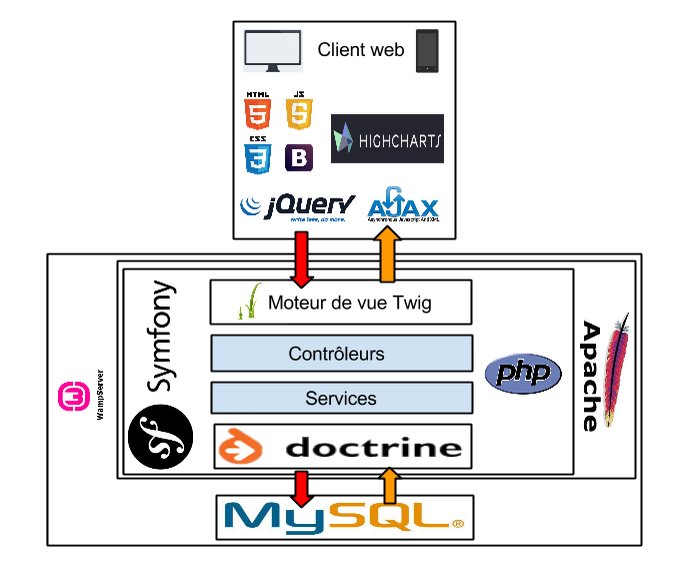
\includegraphics[scale=0.8]{archiTech.png}
\caption{Disposition des Frameworks}
\label{archiTechImg}
\end{figure}


\section{Pr�sentation de l'application}
Dans cette Derni�re partie, nous allons pr�senter � travers quelques captures d'�cran, les principales fonctionnalit�s de notre application.
\begin{itemize}
  \item Authentification
  Cette interface est le point d'entr�e de notre application. Pour s'authentifier, il existe deux moyens, soit � travers un nom d'utilisateur et un mot de passe, soit � travers une adresse mail.
  La figure \ref{loginImg} illustre l'interface d'authentification.

\begin{figure}[!ht]
\centering
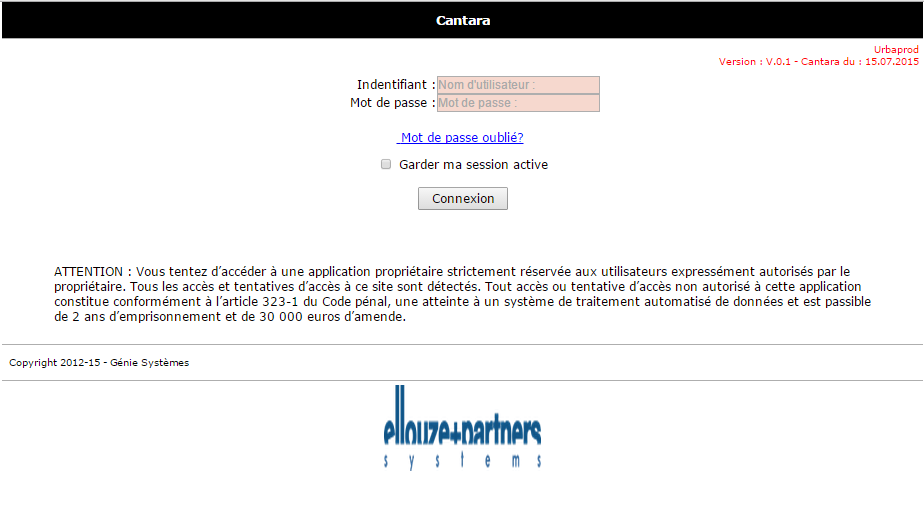
\includegraphics[scale=0.7]{Login.png}
\caption{Interface d'authentification}
\label{loginImg}
\end{figure}

En cas d'�chec, une erreur s'affiche pour indiquer la cause sinon l'utilisateur est renvoy� directement vers l'interface d'accueil.
Ce processus comporte deux phases de s�curit� , la premi�re est l'authentification, c'est � dire la v�rification des donn�es saisies par l'utilisateur afin de lui donner l'acc�s � notre application. La deuxi�me est l'autorisation, elle consiste � v�rifier les droits de cet utilisateur pour acc�der � la ressource demand�e. S'il ne poss�de pas les droits requis, il sera redirig� vers la page d'accueil, si un utilisateur non connect� essaie d'acc�der � une ressource, il sera automatiquement redirig� vers la page d'authentification. La figure \ref{menuImg} met en �vidence la diff�rence entre un r�le collaborateur et un r�le administrateur.
Afin d'impl�menter cette phase, nous avons proc�d� � la s�curisation des URLs.

\begin{figure}[!ht]
\centering
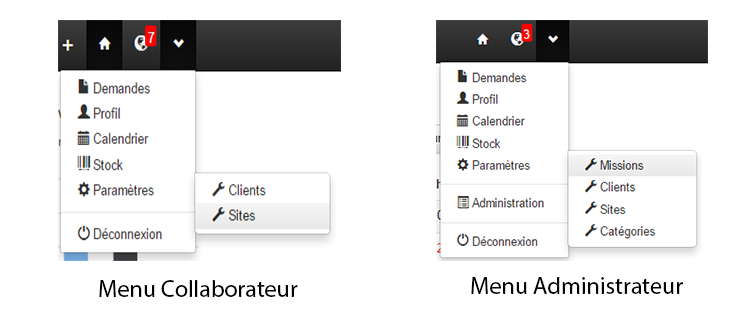
\includegraphics[scale=0.7]{menu.png}
\caption{Diff�rence entre deux r�les}
\label{menuImg}
\end{figure}

  \item Interface d'accueil. \\
  C'est l'interface principale de notre application, elle se pr�sente sous la forme d'une file d'actualit�s compos�e de plusieurs �l�ments simples et faciles � utiliser.
En mettant en place des ic�nes fr�quement utilis�es dans les r�seaux sociaux et dans les applications web ainsi que des interfaces ludiques avec des emplacement bien sp�cifique, nous rendons les vues plus manipulables pour un d�butant permettant de s'y habitu� rapidement.La figure \ref{accueilImg} repr�sente notre �cran d'accueil.

\begin{figure}[!ht]
\centering
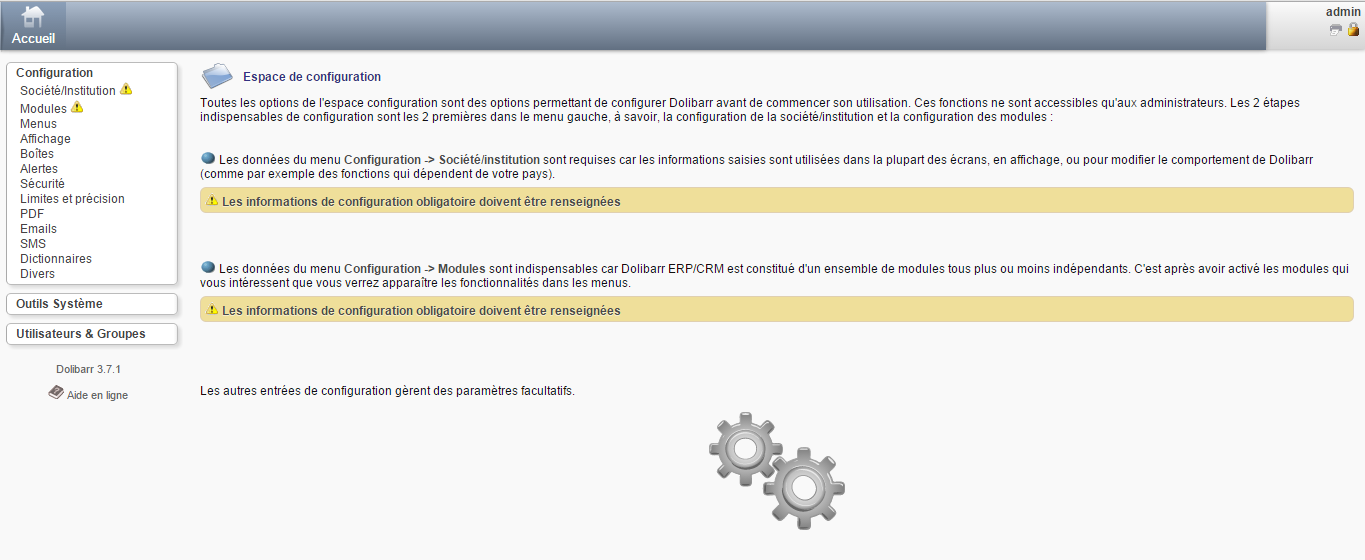
\includegraphics[scale=0.7]{accueil.png}
\caption{Vue compl�te de l'interface d'accueil}
\label{accueilImg}
\end{figure}

Par exemple, pour changer l'�tat de la demande, il suffit d'appuier sur l'�tat actuel de la demande, un "pop-up" appara�t avec un formulaire pour contr�ler l'�tat, et enfin le changement s'effectue sans rechargement de la page. La figure \ref{changerEtatImg} met en �vidence les �tapes cit�es.

\begin{figure}[!ht]
\centering
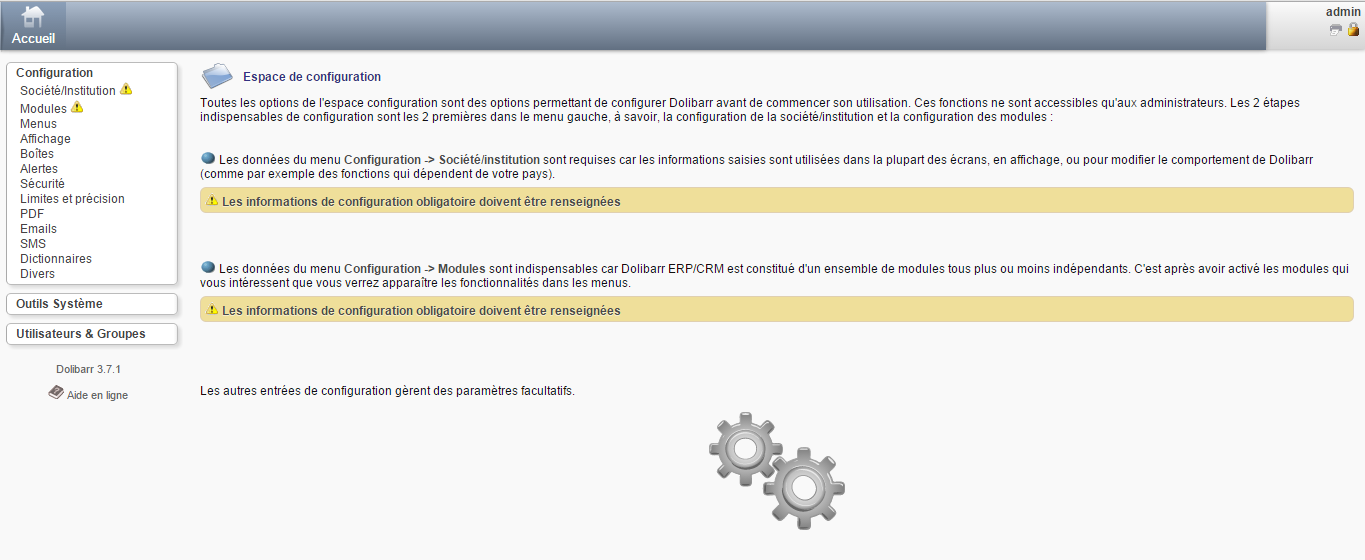
\includegraphics[scale=0.7]{accueil.png}
\caption{Changer l'�tat d'une demande}
\label{changerEtatImg}
\end{figure}

Le graphe � droite de l'�cran montre les demandes trait�es pendant les 3 derniers mois, en choisissant le mois, on aura l'acc�s au �tats des demandes en d�tails i.e. �mise, en cours, annul�e et livr�e.

\begin{figure}[!ht]
\centering
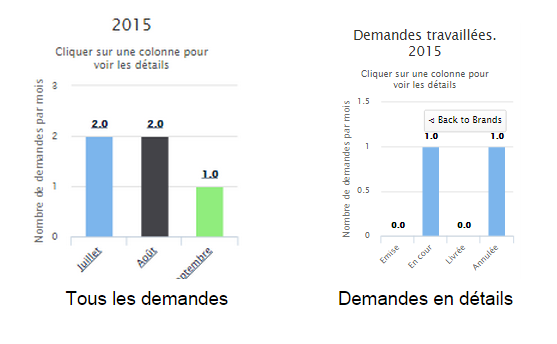
\includegraphics[scale=0.7]{demandeEnDiagramme.png}
\caption{Le graphe des demandes}
\label{demandeEnDiagrammeImg}
\end{figure}

Les composants principaux de cette file d'actualit� sont les demandes. Les collaborateurs en France �mettent une demande � travers un pop-up dans l'accueil.

\begin{figure}[!ht]
\centering
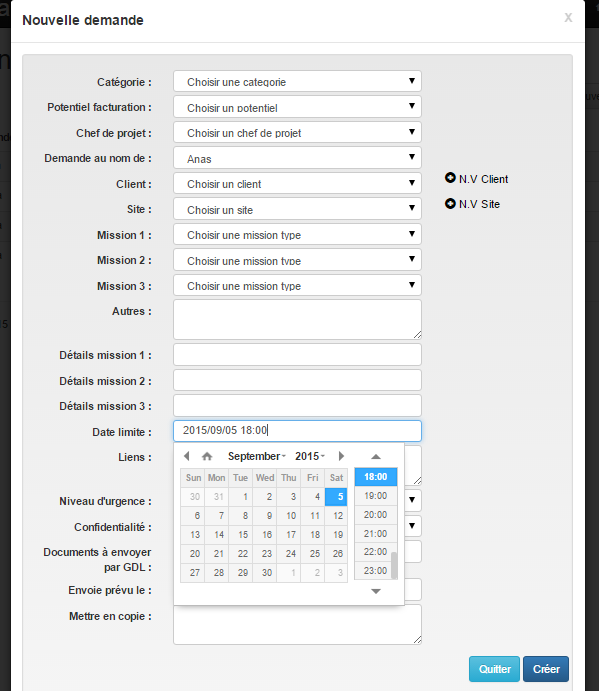
\includegraphics[scale=0.6]{formulaireDemande.png}
\caption{Formulaire de la demande (vue administrateur)}
\label{demandeFormImg}
\end{figure}

La cat�gorie d'une demande est par d�faut de type G�nie des lieux (GDL), seul l'administrateur peut changer la cat�gorie.
Au cour de la cr�ation d'une demande, l'utilisateur, � travers des pop-up, peut ajouter au fur et � mesure des clients et leurs affecter des sites sans besoins de recharger le formulaire de la demande illustr� par la figure \ref{siteFormImg}.

\begin{figure}[!ht]
\centering
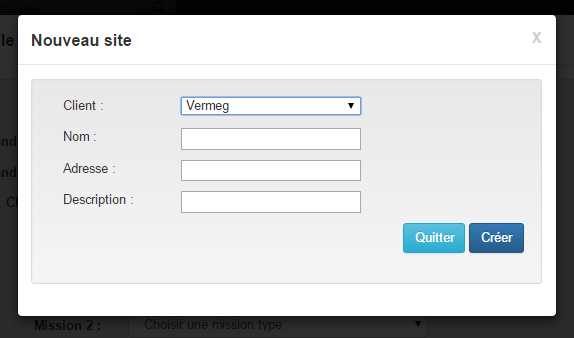
\includegraphics[scale=0.6]{addSite.png}
\caption{Pop-up affectation d'un site}
\label{siteFormImg}
\end{figure}

La demande est �mise dans la file d'actualit� comme introduit par la Figure \ref{demEmisImg}.

\begin{figure}[!ht]
\centering
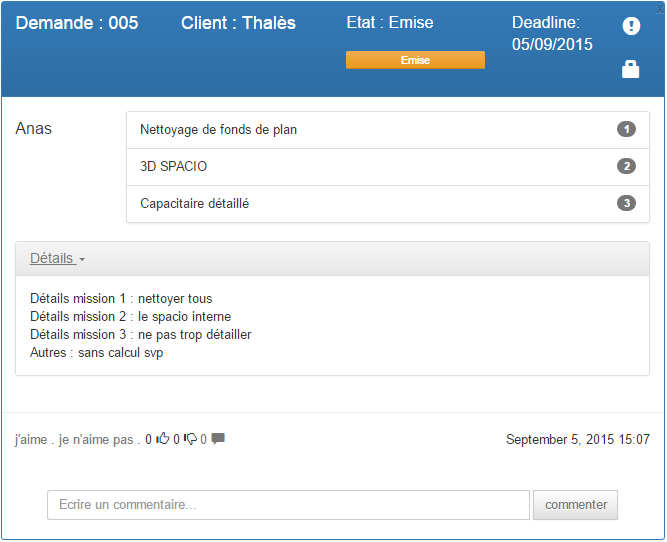
\includegraphics[scale=0.6]{demandeEmise.png}
\caption{Demande �mise}
\label{demEmisImg}
\end{figure}

Une fois la demande �mise, les collaborateurs � Tunis peuvent l'aimer, la commenter, changer son �tat, t�l�charger les fichiers joints etc.
Dans la Figure \ref{demEtCommImg} nous illustrons une demande apr�s plusieurs traitements.

\begin{figure}[!ht]
\centering
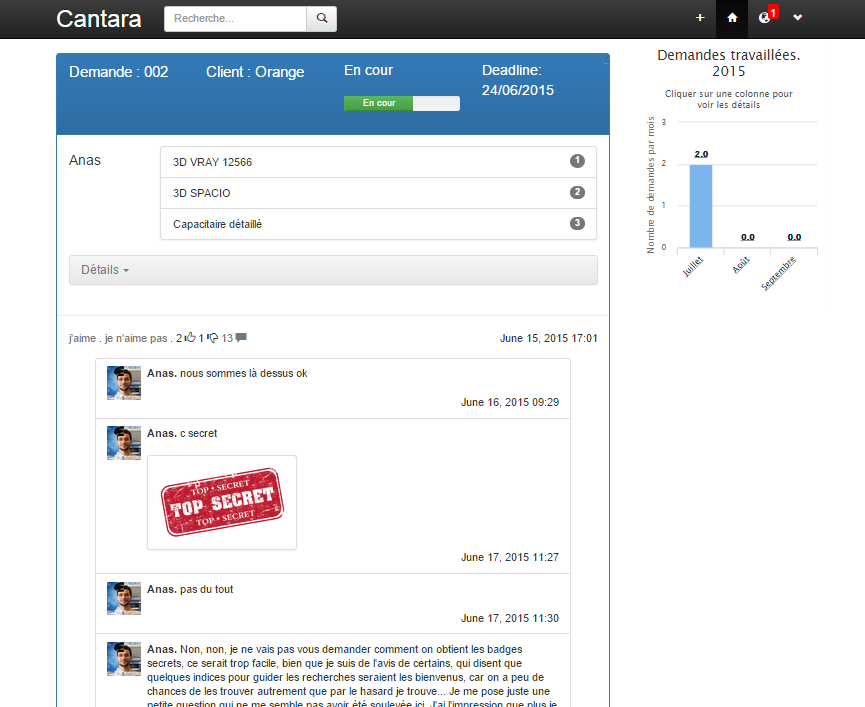
\includegraphics[scale=0.6]{accueilCommentaire.png}
\caption{Demande apr�s traitement}
\label{demEtCommImg}
\end{figure}

  \item Interface �cran commun. \\
  Elle est illustr� par la figure \ref{ecranImg}.C'est une interface affich�e dans un grand �cran devant tous les collaborateurs. Elle donne des informations sp�cifiques afin d'aider dans le suivi des demandes comme l'arriv�e d'un nouveau commentaire ou l'affectation d'un nouveau fichier.

\begin{figure}[!ht]
\centering
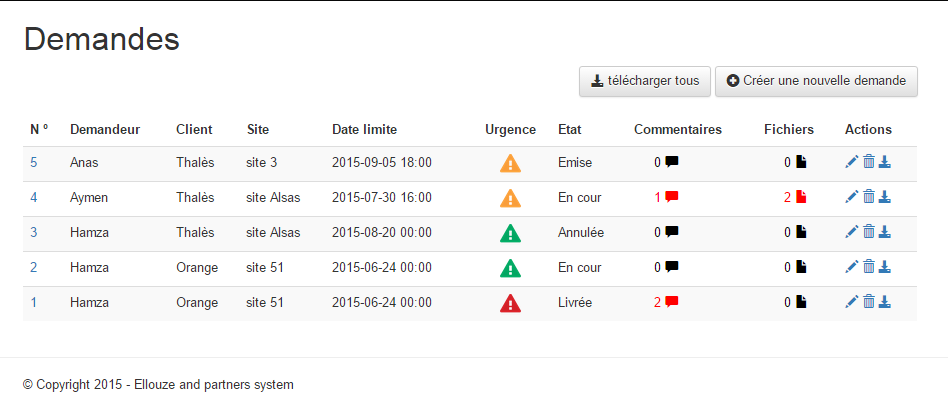
\includegraphics[scale=0.6]{ecranCommun.png}
\caption{Interface �cran commun}
\label{ecranImg}
\end{figure}

Cette interface permet � l'administrateur de cr�er une nouvelle demande ainsi que d'exporter la liste de toutes les demandes dans le syst�me.

  \item Administration des utilisateurs. \\
  Elle permet � l'administrateur toutes les manipulations sur les utilisateurs comme la mise � jour, l'activation ou l'affectation d'un nouveau r�le. Elle est repr�sent� par la figure \ref{userAdmImg}.

\begin{figure}[!ht]
\centering
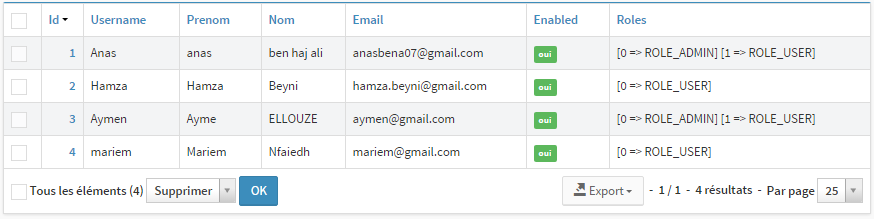
\includegraphics[scale=0.6]{adminUsers.png}
\caption{Interface administration des utilisateurs}
\label{userAdmImg}
\end{figure}  
 
\item Administration des demandes. \\
Elle garantit l'acc�s direct aux donn�es des demandes afin de les modifier � volont� ou les exporter sous plusieurs formats i.e. json, xml, csv.

\begin{figure}[!ht]
\centering
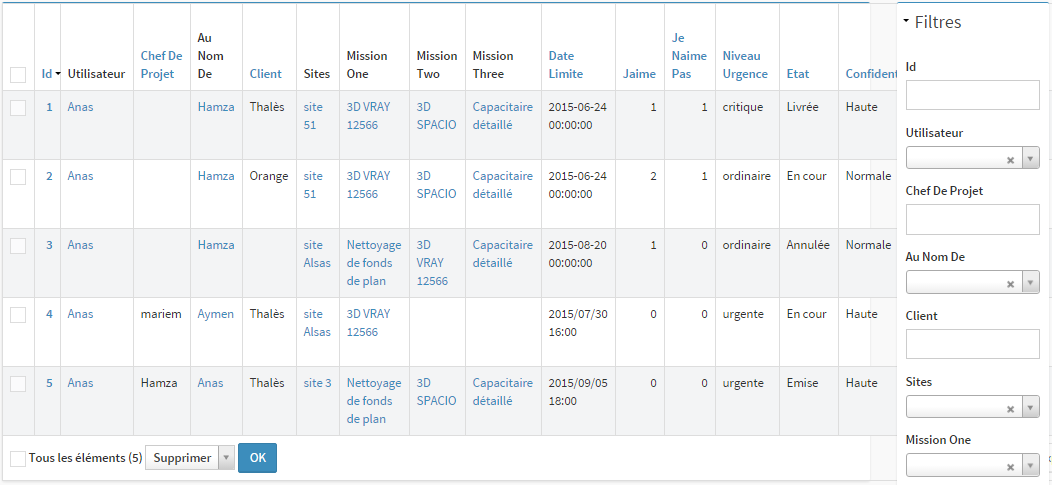
\includegraphics[scale=0.6]{adminDemande.png}
\caption{Interface administration des demandes}
\label{demAdmImg}
\end{figure} 

Cette interface montr�e par la figure \ref{demAdmImg}, assure aussi la filtration des demandes et la recherche des informations selon un ou plusieurs crit�res en m�me temps.
\end{itemize}


\section*{Conclusion}
A travers ce chapitre, nous avons mis en exergue les aspects de la r�alisation de notre travail. Nous avons justifi� le choix de la technologie adapt�e et nous avons pr�sent� notre environnement de travail. Enfin, nous avons concr�tis� le tout avec quelques capture d'�cran de notre application.

%==============================================================================
\end{spacing}



\backmatter
\pagestyle{fancy}
\fancyhf{}
\renewcommand{\chaptermark}[1]{\markboth{Conclusion G�n�rale et Perspectives}{}}
\fancyhead[R]{Conclusion G�n�rale et Perspectives}
\fancyfoot[R]{\thepage}
\renewcommand{\headrulewidth}{0.5pt}
\renewcommand{\footrulewidth}{0pt}
\chapter{Conclusion G�n�rale et Perspectives}
%==============================================================================
\pagestyle{fancy}
\fancyhf{}
\fancyhead[R]{\bfseries\rightmark}
\fancyfoot[R]{\thepage}
\renewcommand{\headrulewidth}{0.5pt}
\renewcommand{\footrulewidth}{0pt}
\renewcommand{\chaptermark}[1]{\markboth{\MakeUppercase{\chaptername~\thechapter. #1 }}{}}
\renewcommand{\sectionmark}[1]{\markright{\thechapter.\thesection~ #1}}

\begin{spacing}{1.2}
%==============================================================================

C'est l'une des parties les plus importantes et pourtant les plus n�glig�es 
du rapport. Ce qu'on \underline{ne veut pas voir} ici, c'est combien ce stage vous a �t� b�n�fique, comment il vous a appris � vous int�grer, � conna�tre le monde du travail, etc.\\
Franchement, personne n'en a rien � faire, du moins dans cette partie. Pour cela, vous 
avez les remerciements et les d�dicaces, vous pourrez vous y exprimer � souhait.\\
La conclusion, c'est tr�s simple : c'est d'abord le r�sum� de ce que vous avez racont�
dans le rapport : vous reprenez votre contribution, en y ajoutant ici les outils que vous 
avez utilis�, votre mani�re de proc�der. Vous pouvez m�me mettre les difficult�s
rencontr�es. En deuxi�me lieu, on y met les perspectives du travail : ce qu'on pourrait 
ajouter � votre application, comment on pourrait l'am�liorer.

%==============================================================================
\end{spacing}


%\bibliographystyle{apalike-fr}
\bibliographystyle{Biblio/unsrt_modif}
\singlespacing
\renewcommand{\bibname}{Bibliographique}

\bibliography{Biblio/aesm_edspia}

\onehalfspacing

\appendix
\setcounter{figure}{0} 
\setcounter{table}{0}
\setcounter{footnote}{0}
\setcounter{equation}{0}
\pagestyle{fancy}
\fancyhf{}
\renewcommand{\chaptermark}[1]{\markboth{\MakeUppercase{#1 }}{}}
\renewcommand{\sectionmark}[1]{\markright{\thesection~ #1}}
\fancyhead[RO]{\bfseries\rightmark}
\fancyhead[LE]{\bfseries\leftmark}
\fancyfoot[RO]{\thepage}
\fancyfoot[LE]{\thepage}
\renewcommand{\headrulewidth}{0.5pt}
\renewcommand{\footrulewidth}{0pt}

\makeatletter
\renewcommand\thefigure{A.\arabic{figure}}
\renewcommand\thetable{A.\arabic{table}} 
\makeatother

\chapter{Annexe : Remarques Diverses}
\graphicspath{{Annexe1/figures/}}
%==========================================================================

%    Annexe

%===========================================================================
\begin{itemize}
\item Un rapport doit toujours �tre bien num�rot�;
\item De pr�f�rence, ne pas utiliser plus que deux couleurs, ni un caract�re fantaisiste; 
\item Essayer de toujours garder votre rapport sobre et professionnel; 
\item Ne jamais utiliser de je ni de on, mais toujours le nous (m�me si tu as tout fait tout seul); 
\item Si on n'a pas de paragraphe 1.2, ne pas mettre de 1.1;
\item TOUJOURS, TOUJOURS faire relire votre rapport � quelqu'un d'autre (de pr�f�rence qui n'est pas du domaine) pour vous corriger les fautes d'orthographe et de fran�ais;
\item Toujours valoriser votre travail : votre contribution doit �tre bien claire et mise en �vidence; 
\item Dans chaque chapitre, on doit trouver une introduction et une conclusion;
\item Ayez toujours un fil conducteur dans votre rapport. Il faut que le lecteur suive un raisonnement bien clair, et trouve la relation entre les diff�rentes parties;
\item Il faut toujours que les abr�viations soient d�finies au moins la premi�re fois o� elles sont utilis�es. Si vous en avez beaucoup, utilisez un glossaire.
\item Vous avez tendance, en d�crivant  l'environnement mat�riel, � parler de votre ordinateur, sur lequel vous avez d�velopp� : ceci est inutile. Dans cette partie, on ne cite que le mat�riel qui a une influence sur votre application. Que vous l'ayez d�velopp� sur Windows Vista ou sur Ubuntu n'a aucune importance;
\item Ne jamais mettre de titres en fin de page; 
\item Essayer toujours d'utiliser des termes fran�ais, et �viter l'anglicisme. Si certains termes  sont plus connus en  anglais, donner leur �quivalent en fran�ais la premi�re fois que vous les utilisez, puis utilisez le mot anglais, mais en italique;
\item �viter les phrases trop longues : clair et concis, c'est la r�gle g�n�rale !\\

\newpage

\textbf{Rappelez vous que votre rapport est le visage de votre travail : un mauvais rapport peut �clipser de l'excellent travail. Alors pr�tez-y l'attention n�cessaire.}

 
\begin{figure}[!ht]\centering

\includegraphics[scale=0.5]{ingenieur.jpg}
\end{figure}
\end{itemize}



\end{document} 